\label{3.5 C8S Answer Key}
\subsection{Answer Key}
\tiny
\renewcommand{\insertclass}{- Class 8}
\renewcommand{\insertsubject}{ - Science}

\begin{frame}[shrink=0.1,label=QPC8QC8S01 - DT - Q7]{Q17 [1. Crop Production and Management]}
\vspace{-0.2cm}
\mcqimgdbottomOneFour{
questionnumber={17}, 
questionTag={C8S01 - DT - Q7}, 
questiontext={Which of the following will you choose to harvest?},
optionA={C8S01 - DT - Q7i.png},
optionAtext={Seed},
optionB={C8S01 - DT - Q7ii.png},
optionBtext={Sprouted plant},
optionC={C8S01 - DT - Q7iii.png},
optionCtext={Sapling},
optionD={C8S01 - DT - Q7iv.png},
optionDtext={Matured plant},
correctoption={D},
}

\begin{minipage}{\linewidth}
\hspace{1cm}
\centering
\tiny
\renewcommand{\arraystretch}{1.25}
\begin{tabular}{|M{1.2cm}|M{0.8cm}|M{0.8cm}|M{0.8cm}|M{0.8cm}|M{0.8cm}|}
\hline
Option & A (\ding{55}) & B (\ding{55}) & C (\ding{55}) & \cellcolor{cellgreen} D (\ding{51}) & E \\ 
\hline
8 A & \highno{31\%} & \highno{8\%} & \highno{0\%} & \highno{62\%} & \highno{0\%} \\ 
 \hline 
8 B & \highno{7\%} & \highno{0\%} & \highno{7\%} & \highgreen{87\%} & \highno{0\%} \\ \hline
\end{tabular}
\end{minipage}

\end{frame}
% \input{4. PPT/6. My Answer/Science/C8/117_C8S - Q17}


\begin{frame}[shrink=0.1,label=QPC8QC8S01 - DT - Q10]{Q27 [1. Crop Production and Management]}
\vspace{-0.2cm}
\mcqimgleftFourOne{
questionnumber={27}, 
questionTag={C8S01 - DT - Q10},
questiontext={Match the following agricultural tools with their uses.},
imgtabletikz = {\renewcommand{\arraystretch}{1.25}
\begin{tabular}{|p{0.25cm}|p{2cm}|p{0.25cm}|p{0.25cm}|p{3cm}|}
\hline
\multicolumn{2}{|c|}{Agricultural tools } & & \multicolumn{2}{|c|}{Uses} \\
\cline{1-2}\cline{4-5}
i & Plough & & a& Weeding \\
\cline{1-2}\cline{4-5}
ii & Hoe & & b & Tilling  \\
\cline{1-2}\cline{4-5}
iii & Seed drill  & & c& Harvesting  \\
\cline{1-2}\cline{4-5}
iv & Sickle & & d& Sowing
\\
\hline
\end{tabular}},
optionA={i-c, ii-d, iii-a, iv-b },
optionB={i-b, ii-c, iii-d, iv-a },
optionC={i-b, ii-a, iii-d, iv-c },
optionD={i-d, ii-a, iii-b, iv-c},
correctoption={C},
leftmini={0.6},
rightmini={0.3},}

\begin{minipage}{\linewidth}
\hspace{1cm}
\centering
\tiny
\renewcommand{\arraystretch}{1.25}
\begin{tabular}{|M{1.2cm}|M{0.8cm}|M{0.8cm}|M{0.8cm}|M{0.8cm}|M{0.8cm}|}
\hline
Option & A (\ding{55}) & B (\ding{55}) & \cellcolor{cellgreen} C (\ding{51}) & D (\ding{55}) & E \\ 
\hline
8 A & \highno{31\%} & \highno{23\%} & \highno{46\%} & \highno{0\%} & \highno{0\%} \\ 
 \hline 
8 B & \highno{13\%} & \highno{20\%} & \highno{53\%} & \highno{13\%} & \highno{0\%} \\ \hline
\end{tabular}
\end{minipage}

\end{frame}
% \input{4. PPT/6. My Answer/Science/C8/117_C8S - Q27}


\begin{frame}[shrink=0.1,label=QPC8QC8S01 - DT - Q9]{Q43 [1. Crop Production and Management]}
\vspace{-0.2cm}
\mcqtextbottomFourOne{
questionnumber={43}, 
questionTag={C8S01 - DT - Q9},
questiontext={Which among the following statement is correct in relation to animal husbandry?},
optionA={Taking care of animals in a large scale by providing them with food and shelter.},
optionB={Hunting wild animals.},
optionC={Providing food and shelter for animals in our home.},
optionD={The process of eliminating animals living in aquatic regions.}, 
correctoption={A},}

\begin{minipage}{\linewidth}
\hspace{1cm}
\centering
\tiny
\renewcommand{\arraystretch}{1.25}
\begin{tabular}{|M{1.2cm}|M{0.8cm}|M{0.8cm}|M{0.8cm}|M{0.8cm}|M{0.8cm}|}
\hline
Option & \cellcolor{cellgreen} A (\ding{51}) & B (\ding{55}) & C (\ding{55}) & D (\ding{55}) & E \\ 
\hline
8 A & \highno{54\%} & \highno{8\%} & \highno{15\%} & \highno{15\%} & \highno{8\%} \\ 
 \hline 
8 B & \highno{73\%} & \highno{13\%} & \highno{13\%} & \highno{0\%} & \highno{0\%} \\ \hline
\end{tabular}
\end{minipage}

\end{frame}
% \input{4. PPT/6. My Answer/Science/C8/117_C8S - Q43}


\begin{frame}[shrink=0.1,label=QPC8QC8S02 - DT - Q7]{Q10 [2. Microorganisms: Friend and Foe]}
\vspace{-0.2cm}
\mcqtextbottomFourOne{
questionnumber={10}, 
questionTag={C8S02 - DT - Q7},
questiontext={What is the role of rhizobium bacteria in the nitrogen cycle?},
optionA={To convert nitrogen gas into ammonia.},
optionB={To release nitrogen gas into the atmospheric air.},
optionC={To convert nitrogen into oxygen and carbon dioxide gases.},
optionD={To break down water molecules into hydrogen and oxygen gases.}, 
correctoption={A},
}

\begin{minipage}{\linewidth}
\hspace{1cm}
\centering
\tiny
\renewcommand{\arraystretch}{1.25}
\begin{tabular}{|M{1.2cm}|M{0.8cm}|M{0.8cm}|M{0.8cm}|M{0.8cm}|M{0.8cm}|}
\hline
Option & \cellcolor{cellgreen} A (\ding{51}) & B (\ding{55}) & C (\ding{55}) & D (\ding{55}) & E \\ 
\hline
8 A & \highred{8\%} & \highno{46\%} & \highno{23\%} & \highno{8\%} & \highno{15\%} \\ 
 \hline 
8 B & \highred{13\%} & \highno{53\%} & \highno{13\%} & \highno{13\%} & \highno{7\%} \\ \hline
\end{tabular}
\end{minipage}

\end{frame}
% \input{4. PPT/6. My Answer/Science/C8/117_C8S - Q10}


\begin{frame}[shrink=0.1,label=QPC8QC8S02 - DT - Q9]{Q18 [2. Microorganisms: Friend and Foe]}
\vspace{-0.2cm}
\mcqimgleftFourOne{
questionnumber={18}, 
questionTag={C8S02 - DT - Q9},
questiontext={Match the reason for transmission of the given human diseases.},
imgtabletikz = {\renewcommand{\arraystretch}{1.25}
\begin{tabular}{|p{0.25cm}|p{2cm}|p{0.25cm}|p{0.25cm}|p{3cm}|}
\hline
\multicolumn{2}{|c|}{Column A  
} & & \multicolumn{2}{|c|}{Column B} \\
\cline{1-2}\cline{4-5}
i & Malaria  & & a& Contaminated water \\
\cline{1-2}\cline{4-5}
ii & Typhoid  & & b & Cough / Sneeze  \\
\cline{1-2}\cline{4-5}
iii & Tuberculosis  & & c& Direct contact
\\
\cline{1-2}\cline{4-5}
iv & Chicken pox
& & d& Mosquito bite 
\\
\hline
\end{tabular}},
optionA={i-c, ii-d, iii-a, iv-b },
optionB={i-b, ii-c, iii-d, iv-a },
optionC={i-b, ii-a, iii-d, iv-c },
optionD={i-d, ii-a, iii-b, iv-c},
correctoption={D},
leftmini={0.6},
rightmini={0.3},
}

\begin{minipage}{\linewidth}
\hspace{1cm}
\centering
\tiny
\renewcommand{\arraystretch}{1.25}
\begin{tabular}{|M{1.2cm}|M{0.8cm}|M{0.8cm}|M{0.8cm}|M{0.8cm}|M{0.8cm}|}
\hline
Option & A (\ding{55}) & B (\ding{55}) & C (\ding{55}) & \cellcolor{cellgreen} D (\ding{51}) & E \\ 
\hline
8 A & \highno{15\%} & \highno{0\%} & \highno{23\%} & \highno{62\%} & \highno{0\%} \\ 
 \hline 
8 B & \highno{0\%} & \highno{7\%} & \highno{13\%} & \highgreen{80\%} & \highno{0\%} \\ \hline
\end{tabular}
\end{minipage}

\end{frame}
% \input{4. PPT/6. My Answer/Science/C8/117_C8S - Q18}


\begin{frame}[shrink=0.1,label=QPC8QC8S02 - DT - Q11]{Q22 [2. Microorganisms: Friend and Foe]}
\vspace{-0.2cm}
\mcqtextbottomOneFour{
questionnumber={22}, 
questionTag={C8S02 - DT - Q11}, 
questiontext={Which of the following diseases cannot be communicated from one person to another?},
optionA={Common cold},
optionB={Diabetes},
optionC={Madras eye},
optionD={Chicken Pox},
correctoption={B},
}

\begin{minipage}{\linewidth}
\hspace{1cm}
\centering
\tiny
\renewcommand{\arraystretch}{1.25}
\begin{tabular}{|M{1.2cm}|M{0.8cm}|M{0.8cm}|M{0.8cm}|M{0.8cm}|M{0.8cm}|}
\hline
Option & A (\ding{55}) & \cellcolor{cellgreen} B (\ding{51}) & C (\ding{55}) & D (\ding{55}) & E \\ 
\hline
8 A & \highno{8\%} & \highgreen{85\%} & \highno{0\%} & \highno{8\%} & \highno{0\%} \\ 
 \hline 
8 B & \highno{0\%} & \highgreen{80\%} & \highno{7\%} & \highno{13\%} & \highno{0\%} \\ \hline
\end{tabular}
\end{minipage}

\end{frame}
% \input{4. PPT/6. My Answer/Science/C8/117_C8S - Q22}


\begin{frame}[shrink=0.1,label=QPC8QC8S05 - DT - Q9]{Q15 [3. Coal and Petroleum]}
\vspace{-0.2cm}
\mcqtextbottomOneFour{
questionnumber={15}, 
questionTag={C8S05 - DT - Q9}, 
questiontext={Identify the fossil fuel that can be easily transported through pipes.},
optionA={Coal},
optionB={Natural gas},
optionC={Petrol},
optionD={Petrochemical},
correctoption={B},
}

\begin{minipage}{\linewidth}
\hspace{1cm}
\centering
\tiny
\renewcommand{\arraystretch}{1.25}
\begin{tabular}{|M{1.2cm}|M{0.8cm}|M{0.8cm}|M{0.8cm}|M{0.8cm}|M{0.8cm}|}
\hline
Option & A (\ding{55}) & \cellcolor{cellgreen} B (\ding{51}) & C (\ding{55}) & D (\ding{55}) & E \\ 
\hline
8 A & \highno{23\%} & \highno{54\%} & \highno{15\%} & \highno{8\%} & \highno{0\%} \\ 
 \hline 
8 B & \highno{7\%} & \highred{33\%} & \highno{53\%} & \highno{7\%} & \highno{0\%} \\ \hline
\end{tabular}
\end{minipage}

\end{frame}
% \input{4. PPT/6. My Answer/Science/C8/117_C8S - Q15}


\begin{frame}[shrink=0.1,label=QPC8QC8S05 - DT - Q3]{Q25 [3. Coal and Petroleum]}
\vspace{-0.2cm}
\mcqtextbottomFourOne{
questionnumber={25}, 
questionTag={C8S05 - DT - Q3},
questiontext={What are fossil fuels?},
optionA={Fuels that are obtained from the earth’s atmosphere.},
optionB={Fuels that are prepared in the laboratories.},
optionC={A type of fuel formed from the renewable energy source of the environment.},
optionD={Fuels that are obtained from the dead remains of plants and animals.}, 
correctoption={D},
}

\begin{minipage}{\linewidth}
\hspace{1cm}
\centering
\tiny
\renewcommand{\arraystretch}{1.25}
\begin{tabular}{|M{1.2cm}|M{0.8cm}|M{0.8cm}|M{0.8cm}|M{0.8cm}|M{0.8cm}|}
\hline
Option & A (\ding{55}) & B (\ding{55}) & C (\ding{55}) & \cellcolor{cellgreen} D (\ding{51}) & E \\ 
\hline
8 A & \highno{8\%} & \highno{23\%} & \highno{31\%} & \highred{38\%} & \highno{0\%} \\ 
 \hline 
8 B & \highno{0\%} & \highno{0\%} & \highno{7\%} & \highgreen{93\%} & \highno{0\%} \\ \hline
\end{tabular}
\end{minipage}

\end{frame}
% \input{4. PPT/6. My Answer/Science/C8/117_C8S - Q25}


\begin{frame}[shrink=0.1,label=QPC8QC8S05 - DT - Q5]{Q33 [3. Coal and Petroleum]}
\vspace{-0.2cm}
\mcqtextsideFourOne{
questionnumber={33},
questionTag = {C8S05 - DT - Q5},
questiontext = {I am black, thick liquid. \\I have an unpleasant smell. \\I am used in road constructions.\\Naphthalene balls are prepared using me. \\Who am I?},
optionA={Coal gas},
optionB={Black gold},
optionC={Coal tar},
optionD={Coke},
correctoption={C},
leftmini = {0.7},
rightmini = {0.2},
}

\begin{minipage}{\linewidth}
\hspace{1cm}
\centering
\tiny
\renewcommand{\arraystretch}{1.25}
\begin{tabular}{|M{1.2cm}|M{0.8cm}|M{0.8cm}|M{0.8cm}|M{0.8cm}|M{0.8cm}|}
\hline
Option & A (\ding{55}) & B (\ding{55}) & \cellcolor{cellgreen} C (\ding{51}) & D (\ding{55}) & E \\ 
\hline
8 A & \highno{15\%} & \highno{8\%} & \highno{62\%} & \highno{15\%} & \highno{0\%} \\ 
 \hline 
8 B & \highno{0\%} & \highno{7\%} & \highgreen{80\%} & \highno{13\%} & \highno{0\%} \\ \hline
\end{tabular}
\end{minipage}

\end{frame}
% \input{4. PPT/6. My Answer/Science/C8/117_C8S - Q33}


\begin{frame}[shrink=0.1,label=QPC8QC8S05 - DT - Q2]{Q45 [3. Coal and Petroleum]}
\vspace{-0.2cm}

\mcqtextbottomOneFour{
questionnumber={45}, 
questionTag={C8S05 - DT - Q2}, 
questiontext={Pick the odd one based on the exhaustible and inexhaustible resources.},
optionA={Water},
optionB={Soil},
optionC={Sunlight},
optionD={Coal},
correctoption={D},
}


\begin{minipage}{\linewidth}
\hspace{1cm}
\centering
\tiny
\renewcommand{\arraystretch}{1.25}
\begin{tabular}{|M{1.2cm}|M{0.8cm}|M{0.8cm}|M{0.8cm}|M{0.8cm}|M{0.8cm}|}
\hline
Option & A (\ding{55}) & B (\ding{55}) & C (\ding{55}) & \cellcolor{cellgreen} D (\ding{51}) & E \\ 
\hline
8 A & \highno{8\%} & \highno{15\%} & \highno{38\%} & \highred{38\%} & \highno{0\%} \\ 
 \hline 
8 B & \highno{0\%} & \highno{20\%} & \highno{20\%} & \highno{60\%} & \highno{0\%} \\ \hline
\end{tabular}
\end{minipage}

\end{frame}
% \input{4. PPT/6. My Answer/Science/C8/117_C8S - Q45}


\begin{frame}[shrink=0.1,label=QPC8QC8S06 - DT - Q2]{Q6 [4. Combustion and Flame]}
\vspace{-0.2cm}
\mcqtextbottomOneFour{
questionnumber={6}, 
questionTag={C8S06 - DT - Q2}, 
questiontext={Find the odd one based on non-combustible substances.},
optionA={Glass},
optionB={Kerosene},
optionC={Paper},
optionD={Wood},
correctoption={A},
}

\begin{minipage}{\linewidth}
\hspace{1cm}
\centering
\tiny
\renewcommand{\arraystretch}{1.25}
\begin{tabular}{|M{1.2cm}|M{0.8cm}|M{0.8cm}|M{0.8cm}|M{0.8cm}|M{0.8cm}|}
\hline
Option & \cellcolor{cellgreen} A (\ding{51}) & B (\ding{55}) & C (\ding{55}) & D (\ding{55}) & E \\ 
\hline
8 A & \highno{62\%} & \highno{15\%} & \highno{23\%} & \highno{0\%} & \highno{0\%} \\ 
 \hline 
8 B & \highgreen{87\%} & \highno{7\%} & \highno{0\%} & \highno{7\%} & \highno{0\%} \\ \hline
\end{tabular}
\end{minipage}

\end{frame}
% \input{4. PPT/6. My Answer/Science/C8/117_C8S - Q6}


\begin{frame}[shrink=0.1,label=QPC8QC8S06 - DT - Q4]{Q7 [4. Combustion and Flame]}
\vspace{-0.2cm}
\mcqtextbottomFourOne{
questionnumber={7}, 
questionTag={C8S06 - DT - Q4},
questiontext={Identify the types of combustion in the given pictures.\\ \smallskip  
\tikzset{every picture/.style={line width=0.75pt,scale=\scalefactor}} 
\hspace{1cm}
\begin{tikzpicture}[x=0.75pt,y=0.75pt,yscale=-1,xscale=1]
\draw (158,101.5) node  {\adjustbox{scale=\scalefactor}{\includegraphics[width=75pt,height=75pt]{C8S06 - DT - Q4i.png}}};
\draw (370,101.5) node  {\adjustbox{scale=\scalefactor}{\includegraphics[width=85pt,height=75pt]{C8S06 - DT - Q4ii.png}}};
\draw (560,101.5) node  {\adjustbox{scale=\scalefactor}{\includegraphics[width=45pt,height=75pt]{C8S06 - DT - Q4iii.png}}};
\draw (121.26,155) node [anchor=north west][inner sep=0.75pt]   [align=left] {Fireworks };
\draw (333.26,155) node [anchor=north west][inner sep=0.75pt]   [align=left] {Forest fire };
\draw (523.26,155) node [anchor=north west][inner sep=0.75pt]   [align=left] {Burning candle };
\draw (85.87,50) node [anchor=north west][inner sep=0.75pt]  [font=\large] [align=left] {1.};
\draw (272.87,50) node [anchor=north west][inner sep=0.75pt]  [font=\large] [align=left] {2.};
\draw (484.87,50) node [anchor=north west][inner sep=0.75pt]  [font=\large] [align=left] {3.};
\end{tikzpicture}},
optionA={1 - Explosive combustion, 2 - Spontaneous combustion, 3 - Rapid combustion},
optionB={1 - Rapid combustion, 2 - Spontaneous combustion, 3 - Explosive combustion},
optionC={1 - Spontaneous combustion, 2 - Rapid combustion, 3 - Explosive combustion},
optionD={1 - Rapid combustion, 2 - Explosive combustion, 3 - Spontaneous combustion}, 
correctoption={A},}

\begin{minipage}{\linewidth}
\hspace{1cm}
\centering
\tiny
\renewcommand{\arraystretch}{1.25}
\begin{tabular}{|M{1.2cm}|M{0.8cm}|M{0.8cm}|M{0.8cm}|M{0.8cm}|M{0.8cm}|}
\hline
Option & \cellcolor{cellgreen} A (\ding{51}) & B (\ding{55}) & C (\ding{55}) & D (\ding{55}) & E \\ 
\hline
8 A & \highgreen{77\%} & \highno{8\%} & \highno{15\%} & \highno{0\%} & \highno{0\%} \\ 
 \hline 
8 B & \highgreen{87\%} & \highno{0\%} & \highno{7\%} & \highno{7\%} & \highno{0\%} \\ \hline
\end{tabular}
\end{minipage}

\end{frame}
% \input{4. PPT/6. My Answer/Science/C8/117_C8S - Q7}


\begin{frame}[shrink=0.1,label=QPC8QC8S06 - DT - Q7]{Q9 [4. Combustion and Flame]}
\vspace{-0.2cm}
\mcqtextbottomOneFour{
questionnumber={9}, 
questionTag={C8S06 - DT - Q7}, 
questiontext={Identify the liquid fuel from the given following.},
optionA={LPG
},
optionB={CNG
},
optionC={Petrol},
optionD={Coke},
correctoption={C},
}

\begin{minipage}{\linewidth}
\hspace{1cm}
\centering
\tiny
\renewcommand{\arraystretch}{1.25}
\begin{tabular}{|M{1.2cm}|M{0.8cm}|M{0.8cm}|M{0.8cm}|M{0.8cm}|M{0.8cm}|}
\hline
Option & A (\ding{55}) & B (\ding{55}) & \cellcolor{cellgreen} C (\ding{51}) & D (\ding{55}) & E \\ 
\hline
8 A & \highno{15\%} & \highno{8\%} & \highno{69\%} & \highno{8\%} & \highno{0\%} \\ 
 \hline 
8 B & \highno{7\%} & \highno{7\%} & \highgreen{80\%} & \highno{7\%} & \highno{0\%} \\ \hline
\end{tabular}
\end{minipage}

\end{frame}
% \input{4. PPT/6. My Answer/Science/C8/117_C8S - Q9}


\begin{frame}[shrink=0.1,label=QPC8QC8S06 - DT - Q9]{Q11 [4. Combustion and Flame]}
\vspace{-0.2cm}
\mcqtextbottomOneFour{
questionnumber={11}, 
questionTag={C8S06 - DT - Q9}, 
questiontext={Which of the following does not produce flame while burning?},
optionA={Coal},
optionB={Candle},
optionC={Camphor},
optionD={LPG},
correctoption={A},
}

\begin{minipage}{\linewidth}
\hspace{1cm}
\centering
\tiny
\renewcommand{\arraystretch}{1.25}
\begin{tabular}{|M{1.2cm}|M{0.8cm}|M{0.8cm}|M{0.8cm}|M{0.8cm}|M{0.8cm}|}
\hline
Option & \cellcolor{cellgreen} A (\ding{51}) & B (\ding{55}) & C (\ding{55}) & D (\ding{55}) & E \\ 
\hline
8 A & \highred{31\%} & \highno{0\%} & \highno{23\%} & \highno{46\%} & \highno{0\%} \\ 
 \hline 
8 B & \highred{27\%} & \highno{0\%} & \highno{33\%} & \highno{40\%} & \highno{0\%} \\ \hline
\end{tabular}
\end{minipage}

\end{frame}
% \input{4. PPT/6. My Answer/Science/C8/117_C8S - Q11}


\begin{frame}[shrink=0.1,label=QPC8QC8S07 - DT - Q10]{Q16 [5. Conservation of Plants and Animals]}
\vspace{-0.2cm}
\mcqtextbottomFourOne{
questionnumber={16}, 
questionTag={C8S07 - DT - Q10},
questiontext={What is the primary purpose of the Project Tiger in India?},
optionA={To promote tourism in tiger reserves.
},
optionB={ To protect and conserve the population of tigers.
},
optionC={To encourage hunting of tigers.
},
optionD={To establish tiger as the national animal of India.
}, 
correctoption={B},
}

\begin{minipage}{\linewidth}
\hspace{1cm}
\centering
\tiny
\renewcommand{\arraystretch}{1.25}
\begin{tabular}{|M{1.2cm}|M{0.8cm}|M{0.8cm}|M{0.8cm}|M{0.8cm}|M{0.8cm}|}
\hline
Option & A (\ding{55}) & \cellcolor{cellgreen} B (\ding{51}) & C (\ding{55}) & D (\ding{55}) & E \\ 
\hline
8 A & \highno{31\%} & \highno{46\%} & \highno{0\%} & \highno{23\%} & \highno{0\%} \\ 
 \hline 
8 B & \highno{13\%} & \highgreen{80\%} & \highno{0\%} & \highno{7\%} & \highno{0\%} \\ \hline
\end{tabular}
\end{minipage}

\end{frame}
% \input{4. PPT/6. My Answer/Science/C8/117_C8S - Q16}


\begin{frame}[shrink=0.1,label=QPC8QC8S07 - DT - Q2]{Q32 [5. Conservation of Plants and Animals]}
\vspace{-0.2cm}
\mcqtextbottomOneFour{
questionnumber={32}, 
questionTag={C8S07 - DT - Q2}, 
questiontext={\rule{80pt}{0.5pt} refers to the variety of living organisms in a specific area. },
optionA={Food chain},
optionB={Biodiversity},
optionC={Botanical garden},
optionD={Animal husbandry},
correctoption={B},}

\begin{minipage}{\linewidth}
\hspace{1cm}
\centering
\tiny
\renewcommand{\arraystretch}{1.25}
\begin{tabular}{|M{1.2cm}|M{0.8cm}|M{0.8cm}|M{0.8cm}|M{0.8cm}|M{0.8cm}|}
\hline
Option & A (\ding{55}) & \cellcolor{cellgreen} B (\ding{51}) & C (\ding{55}) & D (\ding{55}) & E \\ 
\hline
8 A & \highno{31\%} & \highno{46\%} & \highno{8\%} & \highno{8\%} & \highno{8\%} \\ 
 \hline 
8 B & \highno{7\%} & \highgreen{80\%} & \highno{0\%} & \highno{13\%} & \highno{0\%} \\ \hline
\end{tabular}
\end{minipage}

\end{frame}
% \input{4. PPT/6. My Answer/Science/C8/117_C8S - Q32}


\begin{frame}[shrink=0.1,label=QPC8QC8S07 - DT - Q4]{Q34 [5. Conservation of Plants and Animals]}
\vspace{-0.2cm}
\mcqtextbottomTwoTwo{
questionnumber={34}, 
questionTag={C8S07 - DT - Q4},
questiontext={Fill in the blanks.\\i. Species of plants and animals found in a particular place are called \rule{80pt}{0.5pt} species.\\
ii. Plants or animals that might face extinction in the near future are called \rule{80pt}{0.5pt} species.},
optionA={i - Threatened,  ii - Endangered},
optionB={i - Endemic, ii - Extinct },
optionC={i - Endemic, ii - Endangered },
optionD={i - Invasive, ii - Vulnerable }, 
correctoption={C},
}

\begin{minipage}{\linewidth}
\hspace{1cm}
\centering
\tiny
\renewcommand{\arraystretch}{1.25}
\begin{tabular}{|M{1.2cm}|M{0.8cm}|M{0.8cm}|M{0.8cm}|M{0.8cm}|M{0.8cm}|}
\hline
Option & A (\ding{55}) & B (\ding{55}) & \cellcolor{cellgreen} C (\ding{51}) & D (\ding{55}) & E \\ 
\hline
8 A & \highno{8\%} & \highno{54\%} & \highred{31\%} & \highno{8\%} & \highno{0\%} \\ 
 \hline 
8 B & \highno{0\%} & \highno{27\%} & \highno{73\%} & \highno{0\%} & \highno{0\%} \\ \hline
\end{tabular}
\end{minipage}

\end{frame}
% \input{4. PPT/6. My Answer/Science/C8/117_C8S - Q34}


\begin{frame}[shrink=0.1,label=QPC8QC8S07 - DT - Q7]{Q38 [5. Conservation of Plants and Animals]}
\vspace{-0.2cm}
\mcqtextbottomOneFour{
questionnumber={38}, 
questionTag={C8S07 - DT - Q7}, 
questiontext={Which among the following is not a solution for deforestation?},
optionA={Recycling of paper
},
optionB={Desertification
},
optionC={Afforestation
},
optionD={Reforestation
},
correctoption={B},
}

\begin{minipage}{\linewidth}
\hspace{1cm}
\centering
\tiny
\renewcommand{\arraystretch}{1.25}
\begin{tabular}{|M{1.2cm}|M{0.8cm}|M{0.8cm}|M{0.8cm}|M{0.8cm}|M{0.8cm}|}
\hline
Option & A (\ding{55}) & \cellcolor{cellgreen} B (\ding{51}) & C (\ding{55}) & D (\ding{55}) & E \\ 
\hline
8 A & \highno{46\%} & \highred{23\%} & \highno{8\%} & \highno{8\%} & \highno{15\%} \\ 
 \hline 
8 B & \highno{20\%} & \highno{67\%} & \highno{13\%} & \highno{0\%} & \highno{0\%} \\ \hline
\end{tabular}
\end{minipage}

\end{frame}
% \input{4. PPT/6. My Answer/Science/C8/117_C8S - Q38}


\begin{frame}[shrink=0.1,label=QPC8QC8S09 - DT - Q4]{Q21 [6. Reproduction in Animals]}
\vspace{-0.2cm}
\mcqtextbottomFourOne{
questionnumber={21}, 
questionTag={C8S09 - DT - Q4
},
questiontext={Find the correct order in the development of baby formation.},
optionA={Fertilization → Zygote → Embryo → Foetus → Baby
},
optionB={Zygote → Baby → Embryo → Foetus → Fertilisation
},
optionC={Embryo → Foetus → Fertilisation → Zygote → Baby
},
optionD={Baby → Foetus → Embryo → Zygote → Fertilisation
}, 
correctoption={A},
}

\begin{minipage}{\linewidth}
\hspace{1cm}
\centering
\tiny
\renewcommand{\arraystretch}{1.25}
\begin{tabular}{|M{1.2cm}|M{0.8cm}|M{0.8cm}|M{0.8cm}|M{0.8cm}|M{0.8cm}|}
\hline
Option & \cellcolor{cellgreen} A (\ding{51}) & B (\ding{55}) & C (\ding{55}) & D (\ding{55}) & E \\ 
\hline
8 A & \highgreen{85\%} & \highno{8\%} & \highno{0\%} & \highno{8\%} & \highno{0\%} \\ 
 \hline 
8 B & \highgreen{93\%} & \highno{0\%} & \highno{0\%} & \highno{7\%} & \highno{0\%} \\ \hline
\end{tabular}
\end{minipage}

\end{frame}
% \input{4. PPT/6. My Answer/Science/C8/117_C8S - Q21}


\begin{frame}[shrink=0.1,label=QPC8QC8S09 - DT - Q12]{Q26 [6. Reproduction in Animals]}
\vspace{-0.2cm}
\mcqimgbottomOneFour{
questionnumber={26}, 
questionTag={C8S09 - DT - Q12}, 
questiontext={In which among the following animals does external fertilization takes place?},
optionA={C8S09 - DT - Q12i.png},
optionB={C8S09 - DT - Q12ii.png},
optionC={C8S09 - DT - Q12iii.png},
optionD={C8S09 - DT - Q12iv.png},
correctoption={B},
}

\begin{minipage}{\linewidth}
\hspace{1cm}
\centering
\tiny
\renewcommand{\arraystretch}{1.25}
\begin{tabular}{|M{1.2cm}|M{0.8cm}|M{0.8cm}|M{0.8cm}|M{0.8cm}|M{0.8cm}|}
\hline
Option & A (\ding{55}) & \cellcolor{cellgreen} B (\ding{51}) & C (\ding{55}) & D (\ding{55}) & E \\ 
\hline
8 A & \highno{8\%} & \highno{54\%} & \highno{31\%} & \highno{8\%} & \highno{0\%} \\ 
 \hline 
8 B & \highno{0\%} & \highgreen{80\%} & \highno{20\%} & \highno{0\%} & \highno{0\%} \\ \hline
\end{tabular}
\end{minipage}

\end{frame}
% \input{4. PPT/6. My Answer/Science/C8/117_C8S - Q26}


\begin{frame}[shrink=0.1,label=QPC8QC8S09 - DT - Q11]{Q39 [6. Reproduction in Animals]}
\vspace{-0.2cm}

\mcqtextbottomOneFour{
questionnumber={39}, 
questionTag={C8S09 - DT - Q11}, 
questiontext={In which part of the female reproductive system does fertilization occur? },
optionA={Vagina},
optionB={Uterus},
optionC={Ovary},
optionD={Fallopian tube},
correctoption={D},
}


\begin{minipage}{\linewidth}
\hspace{1cm}
\centering
\tiny
\renewcommand{\arraystretch}{1.25}
\begin{tabular}{|M{1.2cm}|M{0.8cm}|M{0.8cm}|M{0.8cm}|M{0.8cm}|M{0.8cm}|}
\hline
Option & A (\ding{55}) & B (\ding{55}) & C (\ding{55}) & \cellcolor{cellgreen} D (\ding{51}) & E \\ 
\hline
8 A & \highno{15\%} & \highno{23\%} & \highno{15\%} & \highno{46\%} & \highno{0\%} \\ 
 \hline 
8 B & \highno{13\%} & \highno{13\%} & \highno{0\%} & \highno{73\%} & \highno{0\%} \\ \hline
\end{tabular}
\end{minipage}

\end{frame}
% \input{4. PPT/6. My Answer/Science/C8/117_C8S - Q39}


\begin{frame}[shrink=0.1,label=QPC8QC8S09 - DT - Q14]{Q50 [6. Reproduction in Animals]}
\vspace{-0.2cm}
\matextbottomFourOne{
myanswerquestion={Label the parent and the bud in each stages of the hydra budding process.},
myanswercontent={\adjustbox{scale=\scalefactor}{\includegraphics[height=3.5cm, width=15cm]{C8S09 - DT - Q14.png}}\\},
questionnumber={50}, 
questionTag={C8S09 - DT - Q14},
questiontext={Why is budding in hydra considered asexual reproduction?},
optionA={Involves two parents to produce a bud},
optionB={Requires fertilization to produce offspring},
optionC={A single parent produces offspring},
optionD={Takes place in water}, 
correctoption={C},
}

\begin{minipage}{\linewidth}
\hspace{1cm}
\centering
\tiny
\renewcommand{\arraystretch}{1.25}
\begin{tabular}{|M{1.2cm}|M{0.8cm}|M{0.8cm}|M{0.8cm}|M{0.8cm}|M{0.8cm}|}
\hline
Option & A (\ding{55}) & B (\ding{55}) & \cellcolor{cellgreen} C (\ding{51}) & D (\ding{55}) & E \\ 
\hline
8 A & \highno{0\%} & \highno{8\%} & \highno{69\%} & \highno{0\%} & \highno{23\%} \\ 
 \hline 
8 B & \highno{7\%} & \highno{7\%} & \highgreen{87\%} & \highno{0\%} & \highno{0\%} \\ \hline
\end{tabular}
\end{minipage}

\end{frame}
\begin{frame}{Q50 - My Answer Responses}
    \vspace{-0.6cm}
    \begin{multicols}{2}

    % Image: Q50_D117214_Science.png - Scaled height: 5.42mm
    \begin{minipage}{\linewidth}
    \RaggedRight\textbf{\tiny \highred{Bhava Nanthan S [E]}} \\ 
    \vspace{4.00pt}\fcolorbox{blue}{white}{\includegraphics[width=5cm]{Q50_D117214_Science.png}}
    \end{minipage}
    \vspace{10pt}

    % Image: Q50_D117226_Science.png - Scaled height: 5.54mm
    \begin{minipage}{\linewidth}
    \RaggedRight\textbf{\tiny \highgreen{Oviya M S [C]}} \\ 
    \vspace{4.00pt}\fcolorbox{blue}{white}{\includegraphics[width=5cm]{Q50_D117226_Science.png}}
    \end{minipage}
    \vspace{10pt}

    % Image: Q50_D117239_Science.png - Scaled height: 5.42mm
    \begin{minipage}{\linewidth}
    \RaggedRight\textbf{\tiny \highred{Inika N [A]}} \\ 
    \vspace{4.00pt}\fcolorbox{blue}{white}{\includegraphics[width=5cm]{Q50_D117239_Science.png}}
    \end{minipage}
    \vspace{10pt}

    % Image: Q50_D117242_Science.png - Scaled height: 5.67mm
    \begin{minipage}{\linewidth}
    \RaggedRight\textbf{\tiny \highgreen{Pranavi T [C]}} \\ 
    \vspace{4.00pt}\fcolorbox{blue}{white}{\includegraphics[width=5cm]{Q50_D117242_Science.png}}
    \end{minipage}
    \vspace{10pt}

    \end{multicols}
\end{frame}



\begin{frame}[shrink=0.1,label=QPC8QC8S09 - DT - Q15]{Q52 [6. Reproduction in Animals]}
\vspace{-0.2cm}
\matextbottomTwoTwo{
myanswerquestion={Look at the given animals and write whether each animal lays eggs or gives birth to young ones.},
myanswercontent={\adjustbox{scale=0.5}{\includegraphics[height=4cm, width=18cm]{C8S09 - DT - Q15.png}}\\},
questionnumber={52}, 
questionTag={C8S09 - DT - Q15},
questiontext={Identify the given animals as viviparous or oviparous and list them in the correct sequence.\\1. Frog, 2. Buffalo, 3. Duck},
optionA={1. Viviparous, 2. Oviparous, 3. Oviparous },
optionB={1. Viviparous, 2. Viviparous, 3. Oviparous },
optionC={1. Oviparous, 2. Viviparous, 3. Oviparous },
optionD={1. Oviparous, 2. Viviparous, 3. Viviparous }, 
correctoption={C},
}

\begin{minipage}{\linewidth}
\hspace{1cm}
\centering
\tiny
\renewcommand{\arraystretch}{1.25}
\begin{tabular}{|M{1.2cm}|M{0.8cm}|M{0.8cm}|M{0.8cm}|M{0.8cm}|M{0.8cm}|}
\hline
Option & A (\ding{55}) & B (\ding{55}) & \cellcolor{cellgreen} C (\ding{51}) & D (\ding{55}) & E \\ 
\hline
8 A & \highno{0\%} & \highno{15\%} & \highno{69\%} & \highno{15\%} & \highno{0\%} \\ 
 \hline 
8 B & \highno{0\%} & \highno{13\%} & \highgreen{80\%} & \highno{7\%} & \highno{0\%} \\ \hline
\end{tabular}
\end{minipage}

\end{frame}

\begin{frame}{Q52 - My Answer Responses}
    \vspace{-0.6cm}
    \begin{multicols}{2}

    % Image: Q52_D117214_Science.png - Scaled height: 4.12mm
    \begin{minipage}{\linewidth}
    \RaggedRight\textbf{\tiny \highgreen{Bhava Nanthan S [C]}} \\ 
    \vspace{4.00pt}\fcolorbox{blue}{white}{\includegraphics[width=6cm]{Q52_D117214_Science.png}}
    \end{minipage}
    \vspace{10pt}

    % Image: Q52_D117226_Science.png - Scaled height: 4.16mm
    \begin{minipage}{\linewidth}
    \RaggedRight\textbf{\tiny \highgreen{Oviya M S [C]}} \\ 
    \vspace{4.00pt}\fcolorbox{blue}{white}{\includegraphics[width=6cm]{Q52_D117226_Science.png}}
    \end{minipage}
    \vspace{10pt}

    % Image: Q52_D117242_Science.png - Scaled height: 4.27mm
    \begin{minipage}{\linewidth}
    \RaggedRight\textbf{\tiny \highgreen{Pranavi T [C]}} \\ 
    \vspace{4.00pt}\fcolorbox{blue}{white}{\includegraphics[width=6cm]{Q52_D117242_Science.png}}
    \end{minipage}
    \vspace{10pt}

    \end{multicols}
\end{frame}





\begin{frame}[shrink=0.1,label=QPC8QC8S10 - DT - Q1]{Q44 [7. Reaching the Age of Adolescence]}
\vspace{-0.2cm}
\mcqimgleftFourOne{
questionnumber={44}, 
questionTag={C8S10 - DT - Q1
},
questiontext={Match the following based on glands and their hormones.},
imgtabletikz = {
\begin{table}[H]
\renewcommand{\arraystretch}{1.25}
\begin{tabular}{|p{0.25cm}|p{2cm}|p{0.25cm}|p{0.25cm}|p{3cm}|}
\hline
\multicolumn{2}{|c|}{Column A} & & \multicolumn{2}{|c|}{Column B} \\
\cline{1-2}\cline{4-5}
i. & Pituitary gland  & & a.& Insulin \\
\cline{1-2}\cline{4-5}
ii. & Pancreas  & & b. &Thyroxine  \\
\cline{1-2}\cline{4-5}
iii. & Thyroid gland  & & c.& Adrenalin \\
\cline{1-2}\cline{4-5}
iv. & Adrenal gland  & & d.& Growth hormone \\
\hline
\end{tabular}
\end {table} },
optionA={i-c, ii-d, iii-a, iv-b},
optionB={i-d, ii-a, iii-b, iv-c},
optionC={i-b, ii-a, iii-d, iv-c},
optionD={i-d, ii-c, iii-b, iv-a},
correctoption={B},
leftmini={0.6},
rightmini={0.3},
}

\begin{minipage}{\linewidth}
\hspace{1cm}
\centering
\tiny
\renewcommand{\arraystretch}{1.25}
\begin{tabular}{|M{1.2cm}|M{0.8cm}|M{0.8cm}|M{0.8cm}|M{0.8cm}|M{0.8cm}|}
\hline
Option & A (\ding{55}) & \cellcolor{cellgreen} B (\ding{51}) & C (\ding{55}) & D (\ding{55}) & E \\ 
\hline
8 A & \highno{15\%} & \highgreen{77\%} & \highno{0\%} & \highno{8\%} & \highno{0\%} \\ 
 \hline 
8 B & \highno{7\%} & \highgreen{87\%} & \highno{7\%} & \highno{0\%} & \highno{0\%} \\ \hline
\end{tabular}
\end{minipage}

\end{frame}
% \input{4. PPT/6. My Answer/Science/C8/117_C8S - Q44}


\begin{frame}[shrink=0.1,label=QPC8QC8S10 - DT - Q8]{Q54 [7. Reaching the Age of Adolescence]}
\vspace{-0.2cm}
\mcqtextbottomOneFour{
questionnumber={54}, 
questionTag={C8S10 - DT - Q8
}, 
questiontext={Maghilan is 13 years old and 144 cm tall. What will be his height as an adult if boys can reach 88\% of their maximum height at this age?},
optionA={152.32 cm 
},
optionB={160.63 cm
},
optionC={163.64 cm 
},
optionD={163 cm
},
correctoption={C},
}

\begin{minipage}{\linewidth}
\hspace{1cm}
\centering
\tiny
\renewcommand{\arraystretch}{1.25}
\begin{tabular}{|M{1.2cm}|M{0.8cm}|M{0.8cm}|M{0.8cm}|M{0.8cm}|M{0.8cm}|}
\hline
Option & A (\ding{55}) & B (\ding{55}) & \cellcolor{cellgreen} C (\ding{51}) & D (\ding{55}) & E \\ 
\hline
8 A & \highno{23\%} & \highno{15\%} & \highno{46\%} & \highno{0\%} & \highno{15\%} \\ 
 \hline 
8 B & \highno{40\%} & \highno{20\%} & \highred{33\%} & \highno{7\%} & \highno{0\%} \\ \hline
\end{tabular}
\end{minipage}

\end{frame}
% \input{4. PPT/6. My Answer/Science/C8/117_C8S - Q54}


\begin{frame}[shrink=10,label=QPC8QC8S10 - DT - Q29]{Q57 [7. Reaching the Age of Adolescence]}
\vspace{-0.2cm}
\matextbottomTwoTwo{
myanswerquestion={Observe the given image carefully and determine whether the baby will be a boy or a girl. Write your answer clearly.},
myanswercontent={
\tikzset{every picture/.style={line width=0.75pt,scale=\scalefactor}} 
\begin{tikzpicture}[x=0.75pt,y=0.75pt,yscale=-1,xscale=1]\
\draw (98.3,64.2) node  {\adjustbox{scale=\scalefactor}{\includegraphics[width=86.85pt,height=35pt]{C8S10 - DT - Q29i.png}}};
\draw (239.9,58.2) node  {\adjustbox{scale=\scalefactor}{\includegraphics[width=45pt,height=46.8pt]{C8S10 - DT - Q29ii.png}}};
\draw    (318.4,65.2) -- (398.2,65.2) ;
\draw [shift={(400.2,65.2)}, rotate = 180] [color={rgb, 255:red, 0; green, 0; blue, 0 }  ][line width=0.75]    (10.93,-4.9) .. controls (6.95,-2.3) and (3.31,-0.67) .. (0,0) .. controls (3.31,0.67) and (6.95,2.3) .. (10.93,4.9)   ;
\draw    (430.4,86) -- (512.2,86) ;
\draw (98.3,164.2) node  {\adjustbox{scale=\scalefactor}{\includegraphics[width=86.85pt,height=35pt]{C8S10 - DT - Q29i.png}}};
\draw (239.9,158.2) node  {\adjustbox{scale=\scalefactor}{\includegraphics[width=45pt,height=46.8pt]{C8S10 - DT - Q29ii.png}}};
\draw    (318.4,165.2) -- (398.2,165.2) ;
\draw [shift={(400.2,165.2)}, rotate = 180] [color={rgb, 255:red, 0; green, 0; blue, 0 }  ][line width=0.75]    (10.93,-4.9) .. controls (6.95,-2.3) and (3.31,-0.67) .. (0,0) .. controls (3.31,0.67) and (6.95,2.3) .. (10.93,4.9)   ;
\draw    (430.4,186) -- (512.2,186) ;
\draw (50,96) node [anchor=north west][inner sep=0.75pt]   [align=left] {X chromosome};
\draw (191.6,96) node [anchor=north west][inner sep=0.75pt]   [align=left] {X chromosome};
\draw (191.6,196) node [anchor=north west][inner sep=0.75pt]   [align=left] {Y chromosome};
\draw (50,196) node [anchor=north west][inner sep=0.75pt]   [align=left] {X chromosome};
\end{tikzpicture} \\
},
questionnumber={57}, 
questionTag={C8S10 - DT - Q29},
questiontext={What determines whether a baby will be male (boy) or female (girl)},
optionA={Mother's chromosomes},
optionB={Father's X or Y chromosomes in sperm},
optionC={Environmental conditions},
optionD={Random chance}, 
correctoption={B},
}

\begin{minipage}{\linewidth}
\hspace{1cm}
\centering
\tiny
\renewcommand{\arraystretch}{1.25}
\begin{tabular}{|M{1.2cm}|M{0.8cm}|M{0.8cm}|M{0.8cm}|M{0.8cm}|M{0.8cm}|}
\hline
Option & A (\ding{55}) & \cellcolor{cellgreen} B (\ding{51}) & C (\ding{55}) & D (\ding{55}) & E \\ 
\hline
8 A & \highno{15\%} & \highgreen{85\%} & \highno{0\%} & \highno{0\%} & \highno{0\%} \\ 
 \hline 
8 B & \highno{0\%} & \highgreen{87\%} & \highno{13\%} & \highno{0\%} & \highno{0\%} \\ \hline
\end{tabular}
\end{minipage}

\end{frame}


\begin{frame}{Q57 - My Answer Responses}
    \vspace{-0.6cm}
    \begin{multicols}{3}

    % Image: Q57_D117220_Science.png - Scaled height: 7.38mm
    \begin{minipage}{\linewidth}
    \RaggedRight\textbf{\tiny \highgreen{Vipulan J R [B]}} \\ 
    \vspace{4.00pt}\fcolorbox{blue}{white}{\includegraphics[width=3.5cm]{Q57_D117220_Science.png}}
    \end{minipage}
    \vspace{10pt}

    % Image: Q57_D117224_Science.png - Scaled height: 7.20mm
    \begin{minipage}{\linewidth}
    \RaggedRight\textbf{\tiny \highgreen{Mirsha K [B]}} \\ 
    \vspace{4.00pt}\fcolorbox{blue}{white}{\includegraphics[width=3.5cm]{Q57_D117224_Science.png}}
    \end{minipage}
    \vspace{10pt}

    % Image: Q57_D117236_Science.png - Scaled height: 7.15mm
    \begin{minipage}{\linewidth}
    \RaggedRight\textbf{\tiny \highgreen{Anushka M [B]}} \\ 
    \vspace{4.00pt}\fcolorbox{blue}{white}{\includegraphics[width=3.5cm]{Q57_D117236_Science.png}}
    \end{minipage}
    \vspace{10pt}

    % Image: Q57_D117239_Science.png - Scaled height: 7.62mm
    \begin{minipage}{\linewidth}
    \RaggedRight\textbf{\tiny \highgreen{Inika N [B]}} \\ 
    \vspace{4.00pt}\fcolorbox{blue}{white}{\includegraphics[width=3.5cm]{Q57_D117239_Science.png}}
    \end{minipage}
    \vspace{10pt}

    % Image: Q57_D117240_Science.png - Scaled height: 7.40mm
    \begin{minipage}{\linewidth}
    \RaggedRight\textbf{\tiny \highgreen{Madhumitha M [B]}} \\ 
    \vspace{4.00pt}\fcolorbox{blue}{white}{\includegraphics[width=3.5cm]{Q57_D117240_Science.png}}
    \end{minipage}
    \vspace{10pt}

    % Image: Q57_D117244_Science.png - Scaled height: 7.15mm
    \begin{minipage}{\linewidth}
    \RaggedRight\textbf{\tiny \highgreen{Shamyuktha Y [B]}} \\ 
    \vspace{4.00pt}\fcolorbox{blue}{white}{\includegraphics[width=3.5cm]{Q57_D117244_Science.png}}
    \end{minipage}
    \vspace{10pt}

    % Image: Q57_D117248_Science.png - Scaled height: 7.24mm
    \begin{minipage}{\linewidth}
    \RaggedRight\textbf{\tiny \highgreen{Dhivyesh R [B]}} \\ 
    \vspace{4.00pt}\fcolorbox{blue}{white}{\includegraphics[width=3.5cm]{Q57_D117248_Science.png}}
    \end{minipage}
    \vspace{10pt}

    \end{multicols}
\end{frame}




\begin{frame}[shrink=0.1,label=QPC8QC8S10 - DT - Q28]{Q60 [7. Reaching the Age of Adolescence]}
\vspace{-0.2cm}
\matextbottomFourOne{
myanswerquestion={Label the stages of human development on the timeline  given below, including adolescence, childhood and adulthood.},
myanswercontent={
\tikzset{every picture/.style={line width=0.75pt,scale=\scalefactor}} 
\centering
\begin{tikzpicture}[x=0.75pt,y=0.75pt,yscale=-1,xscale=1]
\draw    (100,102) -- (563.5,102) ;
\draw    (100,102) -- (100,127) ;
\draw [shift={(100,129)}, rotate = 270] [color={rgb, 255:red, 0; green, 0; blue, 0 }  ][line width=0.75]    (10.93,-3.29) .. controls (6.95,-1.4) and (3.31,-0.3) .. (0,0) .. controls (3.31,0.3) and (6.95,1.4) .. (10.93,3.29)   ;
\draw    (563.5,102) -- (563.5,127) ;
\draw [shift={(563.5,129)}, rotate = 270] [color={rgb, 255:red, 0; green, 0; blue, 0 }  ][line width=0.75]    (10.93,-3.29) .. controls (6.95,-1.4) and (3.31,-0.3) .. (0,0) .. controls (3.31,0.3) and (6.95,1.4) .. (10.93,3.29)   ;
\draw    (331.75,102) -- (331.75,127) ;
\draw [shift={(331.75,129)}, rotate = 270] [color={rgb, 255:red, 0; green, 0; blue, 0 }  ][line width=0.75]    (10.93,-3.29) .. controls (6.95,-1.4) and (3.31,-0.3) .. (0,0) .. controls (3.31,0.3) and (6.95,1.4) .. (10.93,3.29)   ;
\draw    (60.5,170) -- (161.5,170) ;
\draw    (282.5,169.5) -- (383.5,169.5) ;
\draw    (505.5,170) -- (606.5,170) ;
\draw (76,82) node [anchor=north west][inner sep=0.75pt]   [align=left] {0 to 11 years};
\draw (294,83) node [anchor=north west][inner sep=0.75pt]   [align=left] {12 to 19 years};
\draw (520,83) node [anchor=north west][inner sep=0.75pt]   [align=left] {20+ years};
\end{tikzpicture} \\
},
questionnumber={60}, 
questionTag={C8S10 - DT - Q28},
questiontext={Why is adolescence considered a transition period?},
optionA={Since adolescence is the stage when people are born.},
optionB={It bridges childhood and adulthood.},
optionC={Adolescence is the final stage of human development.},
optionD={Adolescence is reversible process.}, 
correctoption={B},
}

\begin{minipage}{\linewidth}
\hspace{1cm}
\centering
\tiny
\renewcommand{\arraystretch}{1.25}
\begin{tabular}{|M{1.2cm}|M{0.8cm}|M{0.8cm}|M{0.8cm}|M{0.8cm}|M{0.8cm}|}
\hline
Option & A (\ding{55}) & \cellcolor{cellgreen} B (\ding{51}) & C (\ding{55}) & D (\ding{55}) & E \\ 
\hline
8 A & \highno{8\%} & \highno{54\%} & \highno{23\%} & \highno{15\%} & \highno{0\%} \\ 
 \hline 
8 B & \highno{0\%} & \highno{60\%} & \highno{27\%} & \highno{13\%} & \highno{0\%} \\ \hline
\end{tabular}
\end{minipage}

\end{frame}


\begin{frame}{Q60 - My Answer Responses}
    \vspace{-0.6cm}
    \begin{multicols}{2}

    % Image: Q60_D117214_Science.png - Scaled height: 4.12mm
    \begin{minipage}{\linewidth}
    \RaggedRight\textbf{\tiny \highred{Bhava Nanthan S [C]}} \\ 
    \vspace{4.00pt}\fcolorbox{blue}{white}{\includegraphics[width=5cm]{Q60_D117214_Science.png}}
    \end{minipage}
    \vspace{10pt}

    % Image: Q60_D117224_Science.png - Scaled height: 3.92mm
    \begin{minipage}{\linewidth}
    \RaggedRight\textbf{\tiny \highgreen{Mirsha K [B]}} \\ 
    \vspace{4.00pt}\fcolorbox{blue}{white}{\includegraphics[width=5cm]{Q60_D117224_Science.png}}
    \end{minipage}
    \vspace{10pt}

    % Image: Q60_D117226_Science.png - Scaled height: 3.97mm
    \begin{minipage}{\linewidth}
    \RaggedRight\textbf{\tiny \highgreen{Oviya M S [B]}} \\ 
    \vspace{4.00pt}\fcolorbox{blue}{white}{\includegraphics[width=5cm]{Q60_D117226_Science.png}}
    \end{minipage}
    \vspace{10pt}

    % Image: Q60_D117236_Science.png - Scaled height: 3.85mm
    \begin{minipage}{\linewidth}
    \RaggedRight\textbf{\tiny \highgreen{Anushka M [B]}} \\ 
    \vspace{4.00pt}\fcolorbox{blue}{white}{\includegraphics[width=5cm]{Q60_D117236_Science.png}}
    \end{minipage}
    \vspace{10pt}


  

    
    % Image: Q60_D117240_Science.png - Scaled height: 3.96mm
    \begin{minipage}{\linewidth}
    \RaggedRight\textbf{\tiny \highgreen{Madhumitha M [B]}} \\ 
    \vspace{4.00pt}\fcolorbox{blue}{white}{\includegraphics[width=5cm]{Q60_D117240_Science.png}}
    \end{minipage}
    \vspace{10pt}

    % Image: Q60_D117242_Science.png - Scaled height: 4.05mm
    \begin{minipage}{\linewidth}
    \RaggedRight\textbf{\tiny \highgreen{Pranavi T [B]}} \\ 
    \vspace{4.00pt}\fcolorbox{blue}{white}{\includegraphics[width=5cm]{Q60_D117242_Science.png}}
    \end{minipage}
    \vspace{10pt}


 \end{multicols}
\end{frame}



\begin{frame}[shrink=0.1,label=QPC8QC8S11 - DT - Q8]{Q14 [8. Force and Pressure]}
\vspace{-0.2cm}
\mcqtextbottomFourOne{
questionnumber={14}, 
questionTag={C8S11 - DT - Q8},
questiontext={Identify the correct answer based on the types of force.},
optionA={Pulling a cart is an example of magnetic force.},
optionB={Repulsion of magnets is an example of electrostatic force.},
optionC={The waterfall is an example of gravitational force.},
optionD={Charging a balloon by rubbing is an example of muscular force.}, 
correctoption={C},
}

\begin{minipage}{\linewidth}
\hspace{1cm}
\centering
\tiny
\renewcommand{\arraystretch}{1.25}
\begin{tabular}{|M{1.2cm}|M{0.8cm}|M{0.8cm}|M{0.8cm}|M{0.8cm}|M{0.8cm}|}
\hline
Option & A (\ding{55}) & B (\ding{55}) & \cellcolor{cellgreen} C (\ding{51}) & D (\ding{55}) & E \\ 
\hline
8 A & \highno{15\%} & \highno{38\%} & \highred{31\%} & \highno{15\%} & \highno{0\%} \\ 
 \hline 
8 B & \highno{7\%} & \highno{7\%} & \highgreen{87\%} & \highno{0\%} & \highno{0\%} \\ \hline
\end{tabular}
\end{minipage}

\end{frame}
% \input{4. PPT/6. My Answer/Science/C8/117_C8S - Q14}


\begin{frame}[shrink=0.1,label=QPC8QC8S11 - DT - Q3]{Q41 [8. Force and Pressure]}
\vspace{-0.2cm}
\mcqtextbottomTwoTwo{
questionnumber={41}, 
questionTag={C8S11 - DT - Q3}, 
questiontext={Identify in which case the box will move on applying force. (Note: The weight of the box is the same in both cases. The force applied by every person is the same.)\\
\tikzset{every picture/.style={line width=0.75pt,scale=\scalefactor}} 
\begin{tikzpicture}[x=0.75pt,y=0.75pt,yscale=-1,xscale=1]
\draw (153,118.96) node  {\adjustbox{scale=\scalefactor}{\includegraphics[width=150pt,height=90pt]{C8S11 - DT - Q3i.png}}};
\draw (433,117.96) node  {\adjustbox{scale=\scalefactor}{\includegraphics[width=180pt,height=90pt]{C8S11 - DT - Q3ii.png}}};
\draw (315,185.93) node [anchor=north west][inner sep=0.75pt]   [align=left] {Force is applied in opposite directions.};
\draw (20,185.93) node [anchor=north west][inner sep=0.75pt][align=left] {Force is applied in the same direction.};
\end{tikzpicture} },
optionA={The box will move in case A.},
optionB={The box will move in case B.},
optionC={Both the boxes will move.},
optionD={Both the boxes will not move.},
correctoption={A},}

\begin{minipage}{\linewidth}
\hspace{1cm}
\centering
\tiny
\renewcommand{\arraystretch}{1.25}
\begin{tabular}{|M{1.2cm}|M{0.8cm}|M{0.8cm}|M{0.8cm}|M{0.8cm}|M{0.8cm}|}
\hline
Option & \cellcolor{cellgreen} A (\ding{51}) & B (\ding{55}) & C (\ding{55}) & D (\ding{55}) & E \\ 
\hline
8 A & \highgreen{77\%} & \highno{15\%} & \highno{8\%} & \highno{0\%} & \highno{0\%} \\ 
 \hline 
8 B & \highgreen{87\%} & \highno{0\%} & \highno{7\%} & \highno{7\%} & \highno{0\%} \\ \hline
\end{tabular}
\end{minipage}

\end{frame}
% \input{4. PPT/6. My Answer/Science/C8/117_C8S - Q41}


\begin{frame}[shrink=0.1,label=QPC8QC8S11 - DT - Q9]{Q46 [8. Force and Pressure]}
\vspace{-0.2cm}
\mcqimgleftFourOne{
questionnumber={46}, 
questionTag={C8S11 - DT - Q9},
questiontext={Which of the following statement is true in relation with the given image?},
imgtabletikz = { {\adjustbox{scale=\scalefactor}{\includegraphics[width=3cm,height=3cm]{C8S11 - DT - Q9.png}}} },
optionA={The pressure is exerted only at the bottom of the container.},
optionB={The pressure exerted at equal depth is equal.},
optionC={The pressure exerted at different depths is equal.},
optionD={The pressure is exerted only at the three points.},
correctoption={B},
leftmini={0.2},
rightmini={0.7},}

\begin{minipage}{\linewidth}
\hspace{1cm}
\centering
\tiny
\renewcommand{\arraystretch}{1.25}
\begin{tabular}{|M{1.2cm}|M{0.8cm}|M{0.8cm}|M{0.8cm}|M{0.8cm}|M{0.8cm}|}
\hline
Option & A (\ding{55}) & \cellcolor{cellgreen} B (\ding{51}) & C (\ding{55}) & D (\ding{55}) & E \\ 
\hline
8 A & \highno{23\%} & \highno{46\%} & \highno{8\%} & \highno{23\%} & \highno{0\%} \\ 
 \hline 
8 B & \highno{47\%} & \highred{20\%} & \highno{7\%} & \highno{27\%} & \highno{0\%} \\ \hline
\end{tabular}
\end{minipage}

\end{frame}
% \input{4. PPT/6. My Answer/Science/C8/117_C8S - Q46}


\begin{frame}[shrink=0.1,label=QPC8QC8S11 - DT - Q7]{Q49 [8. Force and Pressure]}
\vspace{-0.2cm}
\mcqtextbottomOneFour{
questionnumber={49}, 
questionTag={C8S11 - DT - Q7}, 
questiontext={The force acting on an area of 4 $m^2$ is 128 N. Find the pressure acting on that area.},
optionA={62 $Nm^{-2}$ },
optionB={32 $Nm^{-2}$},
optionC={72 $Ncm^{-2}$},
optionD={64 $Nm^{2}$},
correctoption={B},
}

\begin{minipage}{\linewidth}
\hspace{1cm}
\centering
\tiny
\renewcommand{\arraystretch}{1.25}
\begin{tabular}{|M{1.2cm}|M{0.8cm}|M{0.8cm}|M{0.8cm}|M{0.8cm}|M{0.8cm}|}
\hline
Option & A (\ding{55}) & \cellcolor{cellgreen} B (\ding{51}) & C (\ding{55}) & D (\ding{55}) & E \\ 
\hline
8 A & \highno{8\%} & \highno{46\%} & \highno{15\%} & \highno{8\%} & \highno{23\%} \\ 
 \hline 
8 B & \highno{0\%} & \highgreen{80\%} & \highno{7\%} & \highno{13\%} & \highno{0\%} \\ \hline
\end{tabular}
\end{minipage}

\end{frame}
% \input{4. PPT/6. My Answer/Science/C8/117_C8S - Q49}


\begin{frame}[shrink=0.1,label=QPC8QC8S12 - DT - Q10]{Q5 [9. Friction]}
\vspace{-0.2cm}
\mcqimgleftFourOne{
questionnumber={5}, 
questionTag={C8S12 - DT - Q10},
questiontext={Identify the direction of frictional force in the given image. (Hint: Answer the question with the help of the arrow given below).},
imgtabletikz = { {\adjustbox{scale=\scalefactor}{\includegraphics[width=10cm,height=2.5cm]{C8S12 - DT - Q10.png}}} },
optionA={$\longrightarrow$},
optionB={$\uparrow$},
optionC={$\longleftarrow$},
optionD={$\downarrow$},
correctoption={C},
leftmini={0.7},
rightmini={0.2},
}

\begin{minipage}{\linewidth}
\hspace{1cm}
\centering
\tiny
\renewcommand{\arraystretch}{1.25}
\begin{tabular}{|M{1.2cm}|M{0.8cm}|M{0.8cm}|M{0.8cm}|M{0.8cm}|M{0.8cm}|}
\hline
Option & A (\ding{55}) & B (\ding{55}) & \cellcolor{cellgreen} C (\ding{51}) & D (\ding{55}) & E \\ 
\hline
8 A & \highno{38\%} & \highno{15\%} & \highno{46\%} & \highno{0\%} & \highno{0\%} \\ 
 \hline 
8 B & \highno{7\%} & \highno{0\%} & \highgreen{93\%} & \highno{0\%} & \highno{0\%} \\ \hline
\end{tabular}
\end{minipage}

\end{frame}
% \input{4. PPT/6. My Answer/Science/C8/117_C8S - Q5}


\begin{frame}[shrink=0.1,label=QPC8QC8S12 - DT - Q1]{Q31 [9. Friction]}
\vspace{-0.2cm}
\mcqtextbottomOneFour{
questionnumber={31}, 
questionTag={C8S12 - DT - Q1}, 
questiontext={A ball moving on the floor stopped by itself after some time. What caused the ball to come to rest?},
optionA={Muscular force 
},
optionB={Frictional force 
},
optionC={Electrostatic force 
},
optionD={Gravitational force 
},
correctoption={B},
}

\begin{minipage}{\linewidth}
\hspace{1cm}
\centering
\tiny
\renewcommand{\arraystretch}{1.25}
\begin{tabular}{|M{1.2cm}|M{0.8cm}|M{0.8cm}|M{0.8cm}|M{0.8cm}|M{0.8cm}|}
\hline
Option & A (\ding{55}) & \cellcolor{cellgreen} B (\ding{51}) & C (\ding{55}) & D (\ding{55}) & E \\ 
\hline
8 A & \highno{8\%} & \highno{46\%} & \highno{15\%} & \highno{31\%} & \highno{0\%} \\ 
 \hline 
8 B & \highno{0\%} & \highgreen{93\%} & \highno{7\%} & \highno{0\%} & \highno{0\%} \\ \hline
\end{tabular}
\end{minipage}

\end{frame}
% \input{4. PPT/6. My Answer/Science/C8/117_C8S - Q31}


\begin{frame}[shrink=0.1,label=QPC8QC8S12 - DT - Q5]{Q35 [9. Friction]}
\vspace{-0.2cm}
\mcqimgdbottomOneFour{
questionnumber={35}, 
questionTag={C8S12 - DT - Q5}, 
questiontext={Identify the surface in which the friction is very low.},
optionA={C8S12 - DT - Q5i},
optionAtext={Polished inclined},
optionB={C8S12 - DT - Q5ii},
optionBtext={Unpolished },
optionC={C8S12 - DT - Q5iii},
optionCtext={Damaged inclined },
optionD={C8S12 - DT - Q5iv},
optionDtext={Dusty},
correctoption={A},
}

\begin{minipage}{\linewidth}
\hspace{1cm}
\centering
\tiny
\renewcommand{\arraystretch}{1.25}
\begin{tabular}{|M{1.2cm}|M{0.8cm}|M{0.8cm}|M{0.8cm}|M{0.8cm}|M{0.8cm}|}
\hline
Option & \cellcolor{cellgreen} A (\ding{51}) & B (\ding{55}) & C (\ding{55}) & D (\ding{55}) & E \\ 
\hline
8 A & \highgreen{77\%} & \highno{8\%} & \highno{15\%} & \highno{0\%} & \highno{0\%} \\ 
 \hline 
8 B & \highgreen{80\%} & \highno{13\%} & \highno{7\%} & \highno{0\%} & \highno{0\%} \\ \hline
\end{tabular}
\end{minipage}

\end{frame}
% \input{4. PPT/6. My Answer/Science/C8/117_C8S - Q35}


\begin{frame}[shrink=0.1,label=QPC8QC8S12 - DT - Q3]{Q36 [9. Friction]}
\vspace{-0.2cm}
\mcqimgleftFourOne{
questionnumber={36}, 
questionTag={C8S12 - DT - Q3},
questiontext={Match the following based on the types of friction and their example.},
imgtabletikz = {\renewcommand{\arraystretch}{1.5}
\begin{tabular}{|p{0.25cm}|p{2.5cm}|p{0.25cm}|p{0.25cm}|p{4cm}|}
\hline
\multicolumn{2}{|c|}{Column A 
} & & \multicolumn{2}{|c|}{Column B
} \\
\cline{1-2}\cline{4-5}
i & Fluid friction 
& & a& Ball bearing 
\\
\cline{1-2}\cline{4-5}
ii & Sliding friction 
& & b & Pulling a wooden block 
\\
\cline{1-2}\cline{4-5}
iii & Static friction 
& & c& Floating ship 
\\
\cline{1-2}\cline{4-5}
iv & Rolling friction  & & d& Book on the table 
\\
\hline
\end{tabular}},
optionA={i-c, ii-b, iii-d, iv-a },
optionB={i-b, ii-a, iii-d, iv-c },
optionC={i-d, ii-c, iii-b, iv-a },
optionD={i-d, ii-a, iii-b, iv-c},
correctoption={A},
leftmini={0.6},
rightmini={0.3},
}

\begin{minipage}{\linewidth}
\hspace{1cm}
\centering
\tiny
\renewcommand{\arraystretch}{1.25}
\begin{tabular}{|M{1.2cm}|M{0.8cm}|M{0.8cm}|M{0.8cm}|M{0.8cm}|M{0.8cm}|}
\hline
Option & \cellcolor{cellgreen} A (\ding{51}) & B (\ding{55}) & C (\ding{55}) & D (\ding{55}) & E \\ 
\hline
8 A & \highno{54\%} & \highno{8\%} & \highno{15\%} & \highno{23\%} & \highno{0\%} \\ 
 \hline 
8 B & \highgreen{80\%} & \highno{7\%} & \highno{13\%} & \highno{0\%} & \highno{0\%} \\ \hline
\end{tabular}
\end{minipage}

\end{frame}
% \input{4. PPT/6. My Answer/Science/C8/117_C8S - Q36}


\begin{frame}[shrink=0.1,label=QPC8QC8S13 - DT - Q7]{Q20 [10. Sound]}
\vspace{-0.2cm}
\mcqimgbottomOneFour{
questionnumber={20}, 
questionTag={C8S13 - DT - Q7}, 
questiontext={Pick where high-pitched sound is produced.},
optionA={C8S13 - DT - Q7i.png},
optionB={C8S13 - DT - Q7ii.png},
optionC={C8S13 - DT - Q7iii.png},
optionD={C8S13 - DT - Q7iv.png},
correctoption={B},
}

\begin{minipage}{\linewidth}
\hspace{1cm}
\centering
\tiny
\renewcommand{\arraystretch}{1.25}
\begin{tabular}{|M{1.2cm}|M{0.8cm}|M{0.8cm}|M{0.8cm}|M{0.8cm}|M{0.8cm}|}
\hline
Option & A (\ding{55}) & \cellcolor{cellgreen} B (\ding{51}) & C (\ding{55}) & D (\ding{55}) & E \\ 
\hline
8 A & \highno{15\%} & \highno{46\%} & \highno{8\%} & \highno{23\%} & \highno{8\%} \\ 
 \hline 
8 B & \highno{13\%} & \highgreen{80\%} & \highno{7\%} & \highno{0\%} & \highno{0\%} \\ \hline
\end{tabular}
\end{minipage}

\end{frame}
% \input{4. PPT/6. My Answer/Science/C8/117_C8S - Q20}


\begin{frame}[shrink=0.1,label=QPC8QC8S13 - DT - Q2]{Q29 [10. Sound]}
\vspace{-0.2cm}
\mcqtextbottomOneFour{
questionnumber={29}, 
questionTag={C8S13 - DT - Q2}, 
questiontext={In humans, the sound is produced by the \rule{80pt}{0.1pt}.},
optionA={Larynx},
optionB={Windpipe},
optionC={Eardrum},
optionD={Tongue},
correctoption={A},
}

\begin{minipage}{\linewidth}
\hspace{1cm}
\centering
\tiny
\renewcommand{\arraystretch}{1.25}
\begin{tabular}{|M{1.2cm}|M{0.8cm}|M{0.8cm}|M{0.8cm}|M{0.8cm}|M{0.8cm}|}
\hline
Option & \cellcolor{cellgreen} A (\ding{51}) & B (\ding{55}) & C (\ding{55}) & D (\ding{55}) & E \\ 
\hline
8 A & \highgreen{77\%} & \highno{0\%} & \highno{8\%} & \highno{15\%} & \highno{0\%} \\ 
 \hline 
8 B & \highgreen{93\%} & \highno{0\%} & \highno{7\%} & \highno{0\%} & \highno{0\%} \\ \hline
\end{tabular}
\end{minipage}

\end{frame}
% \input{4. PPT/6. My Answer/Science/C8/117_C8S - Q29}


\begin{frame}[shrink=0.1,label=QPC8QC8S13 - DT - Q3]{Q37 [10. Sound]}
\vspace{-0.2cm}
\mcqtextbottomOneFour{
questionnumber={37}, 
questionTag={C8S13 - DT - Q3}, 
questiontext={In which of the following the sound does not travel?},
optionA={Solid},
optionB={Liquid},
optionC={Gas},
optionD={Vacuum},
correctoption={D},
}

\begin{minipage}{\linewidth}
\hspace{1cm}
\centering
\tiny
\renewcommand{\arraystretch}{1.25}
\begin{tabular}{|M{1.2cm}|M{0.8cm}|M{0.8cm}|M{0.8cm}|M{0.8cm}|M{0.8cm}|}
\hline
Option & A (\ding{55}) & B (\ding{55}) & C (\ding{55}) & \cellcolor{cellgreen} D (\ding{51}) & E \\ 
\hline
8 A & \highno{8\%} & \highno{8\%} & \highno{0\%} & \highgreen{85\%} & \highno{0\%} \\ 
 \hline 
8 B & \highno{7\%} & \highno{7\%} & \highno{0\%} & \highgreen{87\%} & \highno{0\%} \\ \hline
\end{tabular}
\end{minipage}

\end{frame}
% \input{4. PPT/6. My Answer/Science/C8/117_C8S - Q37}


\begin{frame}[shrink=13,label=QPC8QC8S13 - DT - Q11]{Q56 [10. Sound]}
\vspace{-0.2cm}

\matextbottomTwoTwo{
myanswerquestion={Circle the image that correctly represents the amplitude.},
myanswercontent={
\tikzset{every picture/.style={line width=0.75pt,scale=0.5}} %set default line width to 0.75pt    
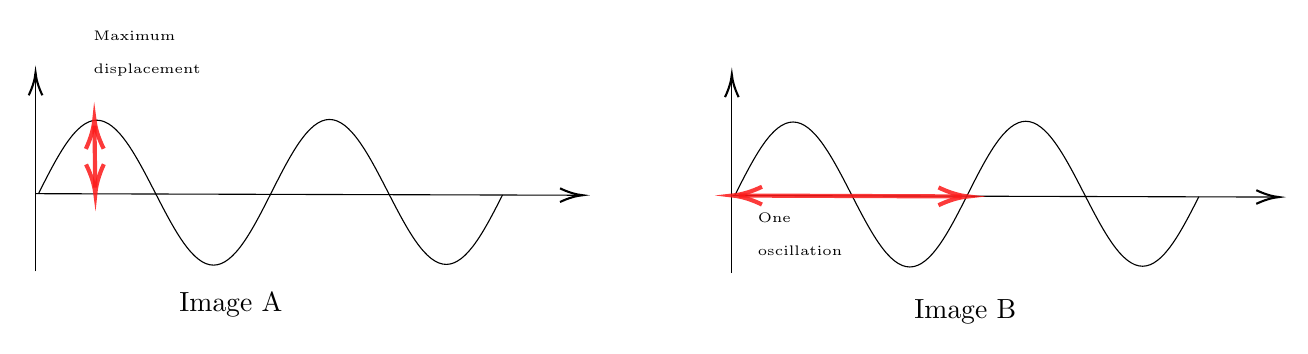
\begin{tikzpicture}[x=0.75pt,y=0.75pt,yscale=-1,xscale=1]
%Shape: Wave [id:dp30988334717784016] 
\draw   (44.83,134.39) .. controls (53.91,116.43) and (62.6,99.33) .. (72.74,99.3) .. controls (82.89,99.27) and (91.69,116.31) .. (100.9,134.22) .. controls (110.1,152.12) and (118.91,169.17) .. (129.05,169.14) .. controls (139.2,169.11) and (147.88,152.01) .. (156.96,134.04) .. controls (166.04,116.08) and (174.73,98.98) .. (184.87,98.95) .. controls (195.02,98.91) and (203.82,115.96) .. (213.03,133.87) .. controls (222.23,151.77) and (231.04,168.82) .. (241.19,168.79) .. controls (251.02,168.76) and (259.49,152.67) .. (268.27,135.31) ;
%Straight Lines [id:da25325835564465193] 
\draw    (43.27,172.1) -- (43.27,78.38) ;
\draw [shift={(43.27,76.38)}, rotate = 90] [color={rgb, 255:red, 0; green, 0; blue, 0 }  ][line width=0.75]    (10.93,-3.29) .. controls (6.95,-1.4) and (3.31,-0.3) .. (0,0) .. controls (3.31,0.3) and (6.95,1.4) .. (10.93,3.29)   ;
%Straight Lines [id:da21631231572462428] 
\draw    (43.58,134.71) -- (304.9,135.46) ;
\draw [shift={(306.9,135.46)}, rotate = 180.16] [color={rgb, 255:red, 0; green, 0; blue, 0 }  ][line width=0.75]    (10.93,-3.29) .. controls (6.95,-1.4) and (3.31,-0.3) .. (0,0) .. controls (3.31,0.3) and (6.95,1.4) .. (10.93,3.29)   ;
%Straight Lines [id:da6532557981814344] 
\draw [color={rgb, 255:red, 252; green, 26; blue, 26 }  ,draw opacity=0.86 ][line width=1.5]    (72.05,131.78) -- (71.66,101.88) ;
\draw [shift={(71.62,98.88)}, rotate = 89.25] [color={rgb, 255:red, 252; green, 26; blue, 26 }  ,draw opacity=0.86 ][line width=1.5]    (14.21,-4.28) .. controls (9.04,-1.82) and (4.3,-0.39) .. (0,0) .. controls (4.3,0.39) and (9.04,1.82) .. (14.21,4.28)   ;
\draw [shift={(72.08,134.78)}, rotate = 269.25] [color={rgb, 255:red, 252; green, 26; blue, 26 }  ,draw opacity=0.86 ][line width=1.5]    (14.21,-4.28) .. controls (9.04,-1.82) and (4.3,-0.39) .. (0,0) .. controls (4.3,0.39) and (9.04,1.82) .. (14.21,4.28)   ;
%Shape: Wave [id:dp5256617175372751] 
\draw   (380.3,135.28) .. controls (389.38,117.32) and (398.06,100.22) .. (408.21,100.18) .. controls (418.35,100.15) and (427.16,117.2) .. (436.36,135.1) .. controls (445.57,153.01) and (454.37,170.06) .. (464.52,170.03) .. controls (474.66,169.99) and (483.35,152.89) .. (492.43,134.93) .. controls (501.51,116.97) and (510.19,99.86) .. (520.34,99.83) .. controls (530.48,99.8) and (539.29,116.85) .. (548.49,134.75) .. controls (557.7,152.66) and (566.5,169.71) .. (576.65,169.67) .. controls (586.49,169.64) and (594.96,153.56) .. (603.74,136.2) ;
%Straight Lines [id:da21018279548408225] 
\draw    (378.74,172.98) -- (378.74,79.26) ;
\draw [shift={(378.74,77.26)}, rotate = 90] [color={rgb, 255:red, 0; green, 0; blue, 0 }  ][line width=0.75]    (10.93,-3.29) .. controls (6.95,-1.4) and (3.31,-0.3) .. (0,0) .. controls (3.31,0.3) and (6.95,1.4) .. (10.93,3.29)   ;
%Straight Lines [id:da38446066584415917] 
\draw    (379.05,135.6) -- (640.36,136.34) ;
\draw [shift={(642.36,136.35)}, rotate = 180.16] [color={rgb, 255:red, 0; green, 0; blue, 0 }  ][line width=0.75]    (10.93,-3.29) .. controls (6.95,-1.4) and (3.31,-0.3) .. (0,0) .. controls (3.31,0.3) and (6.95,1.4) .. (10.93,3.29)   ;
%Straight Lines [id:da5391653616172787] 
\draw [color={rgb, 255:red, 252; green, 26; blue, 26 }  ,draw opacity=0.86 ][line width=1.5]    (489.51,136.04) -- (382.05,135.61) ;
\draw [shift={(379.05,135.6)}, rotate = 0.23] [color={rgb, 255:red, 252; green, 26; blue, 26 }  ,draw opacity=0.86 ][line width=1.5]    (14.21,-4.28) .. controls (9.04,-1.82) and (4.3,-0.39) .. (0,0) .. controls (4.3,0.39) and (9.04,1.82) .. (14.21,4.28)   ;
\draw [shift={(492.51,136.05)}, rotate = 180.23] [color={rgb, 255:red, 252; green, 26; blue, 26 }  ,draw opacity=0.86 ][line width=1.5]    (14.21,-4.28) .. controls (9.04,-1.82) and (4.3,-0.39) .. (0,0) .. controls (4.3,0.39) and (9.04,1.82) .. (14.21,4.28)   ;

% Text Node
\draw (70,55) node [anchor=north west][inner sep=0.75pt]   [align=left] {{\tiny Maximum }\\{\tiny displacement }};
% Text Node
\draw (111.27,181.05) node [anchor=north west][inner sep=0.75pt]   [align=left] {Image A};
% Text Node
\draw (390,142.63) node [anchor=north west][inner sep=0.75pt]   [align=left] {{\tiny One }\\{\tiny oscillation }};
% Text Node
\draw (465.39,184.59) node [anchor=north west][inner sep=0.75pt]   [align=left] {Image B};
\end{tikzpicture} \\
},
questionnumber={56}, 
questionTag={C8S13 - DT - Q11}, 
questiontext={Whose amplitude is high?\\
\tikzset{every picture/.style={line width=0.75pt,scale=0.5}} %set default line width to 0.75pt    
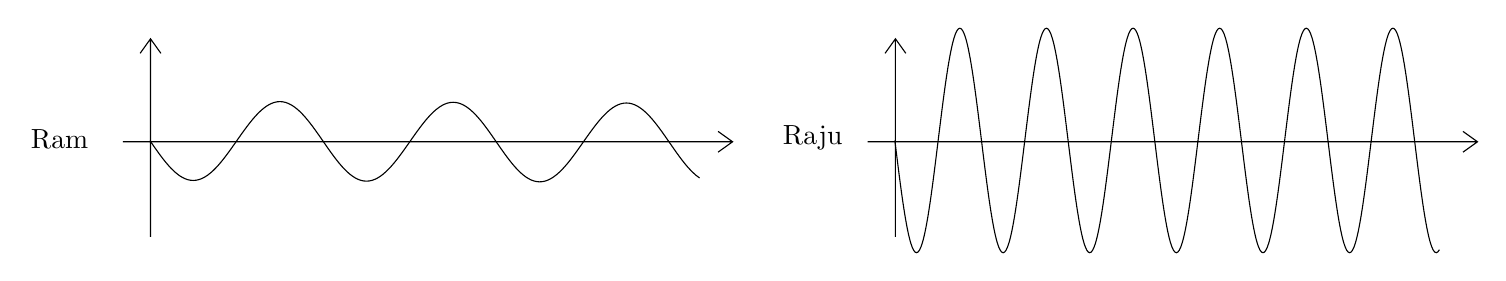
\begin{tikzpicture}[x=0.75pt,y=0.75pt,yscale=-1,xscale=1]
%Shape: Wave [id:dp1150601366869346] 
\draw   (82.76,107.85) .. controls (89.53,117.65) and (96.02,126.98) .. (103.57,127.01) .. controls (111.12,127.04) and (117.65,117.76) .. (124.49,108.01) .. controls (131.32,98.27) and (137.86,88.99) .. (145.41,89.02) .. controls (152.96,89.05) and (159.44,98.38) .. (166.22,108.18) .. controls (173,117.99) and (179.48,127.32) .. (187.03,127.35) .. controls (194.58,127.38) and (201.12,118.1) .. (207.95,108.35) .. controls (214.78,98.6) and (221.32,89.32) .. (228.87,89.35) .. controls (236.42,89.38) and (242.91,98.71) .. (249.68,108.52) .. controls (256.46,118.32) and (262.94,127.65) .. (270.49,127.68) .. controls (278.04,127.71) and (284.58,118.43) .. (291.41,108.68) .. controls (298.25,98.94) and (304.78,89.66) .. (312.33,89.69) .. controls (319.89,89.72) and (326.37,99.05) .. (333.14,108.85) .. controls (337.94,115.78) and (342.58,122.48) .. (347.56,125.82) ;
%Shape: Axis 2D [id:dp7745247508674722] 
\draw  (69.68,108.38) -- (363.47,108.38)(83.03,58.76) -- (83.03,154.18) (356.47,103.38) -- (363.47,108.38) -- (356.47,113.38) (78.03,65.76) -- (83.03,58.76) -- (88.03,65.76)  ;
%Shape: Wave [id:dp880200418505847] 
\draw   (441.65,107.74) .. controls (445.05,135.44) and (448.31,161.82) .. (452.08,161.82) .. controls (455.86,161.82) and (459.11,135.44) .. (462.51,107.74) .. controls (465.92,80.04) and (469.17,53.67) .. (472.95,53.67) .. controls (476.72,53.67) and (479.98,80.04) .. (483.38,107.74) .. controls (486.78,135.44) and (490.04,161.82) .. (493.81,161.82) .. controls (497.59,161.82) and (500.84,135.44) .. (504.25,107.74) .. controls (507.65,80.04) and (510.9,53.67) .. (514.68,53.67) .. controls (518.45,53.67) and (521.71,80.04) .. (525.11,107.74) .. controls (528.51,135.44) and (531.77,161.82) .. (535.54,161.82) .. controls (539.32,161.82) and (542.57,135.44) .. (545.98,107.74) .. controls (549.38,80.04) and (552.63,53.67) .. (556.41,53.67) .. controls (560.19,53.67) and (563.44,80.04) .. (566.84,107.74) .. controls (570.25,135.44) and (573.5,161.82) .. (577.28,161.82) .. controls (581.05,161.82) and (584.31,135.44) .. (587.71,107.74) .. controls (591.11,80.04) and (594.37,53.67) .. (598.14,53.67) .. controls (601.92,53.67) and (605.17,80.04) .. (608.58,107.74) .. controls (611.98,135.44) and (615.23,161.82) .. (619.01,161.82) .. controls (622.78,161.82) and (626.04,135.44) .. (629.44,107.74) .. controls (632.84,80.04) and (636.1,53.67) .. (639.87,53.67) .. controls (643.65,53.67) and (646.9,80.04) .. (650.31,107.74) .. controls (653.71,135.44) and (656.96,161.82) .. (660.74,161.82) .. controls (664.52,161.82) and (667.77,135.44) .. (671.17,107.74) .. controls (674.58,80.04) and (677.83,53.67) .. (681.61,53.67) .. controls (685.38,53.67) and (688.64,80.04) .. (692.04,107.74) .. controls (695.44,135.44) and (698.7,161.82) .. (702.47,161.82) .. controls (702.99,161.82) and (703.5,161.32) .. (704,160.39) ;
%Shape: Axis 2D [id:dp6911850965481281] 
\draw  (428.57,108.38) -- (722.36,108.38)(441.93,58.76) -- (441.93,154.18) (715.36,103.38) -- (722.36,108.38) -- (715.36,113.38) (436.93,65.76) -- (441.93,58.76) -- (446.93,65.76)  ;

% Text Node
\draw (386.42,99.42) node [anchor=north west][inner sep=0.75pt]   [align=left] {Raju};
% Text Node
\draw (24.11,101.33) node [anchor=north west][inner sep=0.75pt]   [align=left] {Ram};
\end{tikzpicture}
},
optionA={Raju’s amplitude is high},
optionB={Ram’s amplitude is high},
optionC={Both amplitudes are low},
optionD={Both amplitudes are high},
correctoption={A},
}


\begin{minipage}{\linewidth}
\hspace{1cm}
\centering
\tiny
\renewcommand{\arraystretch}{1.25}
\begin{tabular}{|M{1.2cm}|M{0.8cm}|M{0.8cm}|M{0.8cm}|M{0.8cm}|M{0.8cm}|}
\hline
Option & \cellcolor{cellgreen} A (\ding{51}) & B (\ding{55}) & C (\ding{55}) & D (\ding{55}) & E \\ 
\hline
8 A & \highno{69\%} & \highno{15\%} & \highno{15\%} & \highno{0\%} & \highno{0\%} \\ 
 \hline 
8 B & \highno{73\%} & \highno{13\%} & \highno{13\%} & \highno{0\%} & \highno{0\%} \\ \hline
\end{tabular}
\end{minipage}

\end{frame}


\begin{frame}{Q56 - My Answer Responses}
    \vspace{-0.6cm}
    \begin{multicols}{2}

    % Image: Q56_D117214_Science.png - Scaled height: 3.96mm
    \begin{minipage}{\linewidth}
    \RaggedRight\textbf{\tiny \highgreen{Bhava Nanthan S [A]}} \\ 
    \vspace{4.00pt}\fcolorbox{blue}{white}{\includegraphics[width=5cm]{Q56_D117214_Science.png}}
    \end{minipage}
    \vspace{10pt}

    % Image: Q56_D117233_Science.png - Scaled height: 3.93mm
    \begin{minipage}{\linewidth}
    \RaggedRight\textbf{\tiny \highgreen{Rithvik Kanishkar S [A]}} \\ 
    \vspace{4.00pt}\fcolorbox{blue}{white}{\includegraphics[width=5cm]{Q56_D117233_Science.png}}
    \end{minipage}
    \vspace{10pt}

    % Image: Q56_D117237_Science.png - Scaled height: 3.95mm
    \begin{minipage}{\linewidth}
    \RaggedRight\textbf{\tiny \highgreen{Cathrine Bertina F [A]}} \\ 
    \vspace{4.00pt}\fcolorbox{blue}{white}{\includegraphics[width=5cm]{Q56_D117237_Science.png}}
    \end{minipage}
    \vspace{10pt}

    % Image: Q56_D117241_Science.png - Scaled height: 3.99mm
    \begin{minipage}{\linewidth}
    \RaggedRight\textbf{\tiny \highgreen{Nidharshana D [A]}} \\ 
    \vspace{4.00pt}\fcolorbox{blue}{white}{\includegraphics[width=5cm]{Q56_D117241_Science.png}}
    \end{minipage}
    \vspace{10pt}

    % Image: Q56_D117245_Science.png - Scaled height: 3.95mm
    \begin{minipage}{\linewidth}
    \RaggedRight\textbf{\tiny \highgreen{Sowbarnika S [A]}} \\ 
    \vspace{4.00pt}\fcolorbox{blue}{white}{\includegraphics[width=5cm]{Q56_D117245_Science.png}}
    \end{minipage}
    \vspace{10pt}

    \end{multicols}
\end{frame}




\begin{frame}[shrink=0.1,label=QPC8QC8S14 - DT - Q7]{Q23 [11. Chemical Effects of Electric Current]}
\vspace{-0.2cm}
\mcqtextbottomFourOne{
questionnumber={23}, 
questionTag={C8S14 - DT - Q7},
questiontext={What is electroplating?},
optionA={The process of using electricity to deposit a layer of metal onto an object.
},
optionB={The process of coating a metal object with a layer of grease.
},
optionC={The process of producing electricity from metal objects.
},
optionD={The process of extracting one metal from its ore.
}, 
correctoption={A},
}

\begin{minipage}{\linewidth}
\hspace{1cm}
\centering
\tiny
\renewcommand{\arraystretch}{1.25}
\begin{tabular}{|M{1.2cm}|M{0.8cm}|M{0.8cm}|M{0.8cm}|M{0.8cm}|M{0.8cm}|}
\hline
Option & \cellcolor{cellgreen} A (\ding{51}) & B (\ding{55}) & C (\ding{55}) & D (\ding{55}) & E \\ 
\hline
8 A & \highgreen{85\%} & \highno{8\%} & \highno{8\%} & \highno{0\%} & \highno{0\%} \\ 
 \hline 
8 B & \highgreen{87\%} & \highno{7\%} & \highno{7\%} & \highno{0\%} & \highno{0\%} \\ \hline
\end{tabular}
\end{minipage}

\end{frame}
% \input{4. PPT/6. My Answer/Science/C8/117_C8S - Q23}


\begin{frame}[shrink=0.1,label=QPC8QC8S14 - DT - Q19]{Q28 [11. Chemical Effects of Electric Current]}
\vspace{-0.2cm}

\mcqtextbottomTwoTwo{
questionnumber={28}, 
questionTag={C8S14 - DT - Q19}, 
questiontext={Why should electrical switches not be touched directly with wet hands?},
optionA={To maintain the cleanliness of the switch.},
optionB={To avoid electric shock.},
optionC={Water is a bad conductor of electricity.},
optionD={Wet hands acts an insulator to electricity.},
correctoption={B},
}

\begin{minipage}{\linewidth}
\hspace{1cm}
\centering
\tiny
\renewcommand{\arraystretch}{1.25}
\begin{tabular}{|M{1.2cm}|M{0.8cm}|M{0.8cm}|M{0.8cm}|M{0.8cm}|M{0.8cm}|}
\hline
Option & A (\ding{55}) & \cellcolor{cellgreen} B (\ding{51}) & C (\ding{55}) & D (\ding{55}) & E \\ 
\hline
8 A & \highno{8\%} & \highgreen{77\%} & \highno{15\%} & \highno{0\%} & \highno{0\%} \\ 
 \hline 
8 B & \highno{7\%} & \highgreen{93\%} & \highno{0\%} & \highno{0\%} & \highno{0\%} \\ \hline
\end{tabular}
\end{minipage}

\end{frame}
% \input{4. PPT/6. My Answer/Science/C8/117_C8S - Q28}


\begin{frame}[shrink=0.1,label=QPC8QC8S14 - DT - Q3]{Q30 [11. Chemical Effects of Electric Current]}
\vspace{-0.2cm}
\mcqimgleftFourOne{
questionnumber={30}, 
questionTag={C8S14 - DT - Q3},
questiontext={Which liquid can be used in the given circuit to make the LED bulb glow?},
imgtabletikz = {

\tikzset{every picture/.style={line width=0.75pt,scale=\scalefactor}} %set default line width to 0.75pt        

\begin{tikzpicture}[x=0.75pt,y=0.75pt,yscale=-1,xscale=1]
%uncomment if require: \path (0,300); %set diagram left start at 0, and has height of 300

%Image [id:dp8658295316073186] 
\draw (176,123.5) node  {\adjustbox{scale=\scalefactor}{\includegraphics[width=114pt,height=95.25pt]{C8S14 - DT - Q3i.png}}};
%Straight Lines [id:da5178347498289086] 
\draw [color={rgb, 255:red, 13; green, 13; blue, 13 }  ,draw opacity=1 ][line width=1.5]    (154,179) -- (293,179) ;
\draw [shift={(297,179)}, rotate = 180] [fill={rgb, 255:red, 13; green, 13; blue, 13 }  ,fill opacity=1 ][line width=0.08]  [draw opacity=0] (13.4,-6.43) -- (0,0) -- (13.4,6.44) -- (8.9,0) -- cycle    ;


% Text Node
\draw (311,170) node [anchor=north west][inner sep=0.75pt]   [align=left] {?};


\end{tikzpicture}
},
optionA={Distilled water
},
optionB={Orange juice
},
optionC={Oil
},
optionD={No liquid is required
},
correctoption={B},
leftmini={0.5},
rightmini={0.4},
}

\begin{minipage}{\linewidth}
\hspace{1cm}
\centering
\tiny
\renewcommand{\arraystretch}{1.25}
\begin{tabular}{|M{1.2cm}|M{0.8cm}|M{0.8cm}|M{0.8cm}|M{0.8cm}|M{0.8cm}|}
\hline
Option & A (\ding{55}) & \cellcolor{cellgreen} B (\ding{51}) & C (\ding{55}) & D (\ding{55}) & E \\ 
\hline
8 A & \highno{46\%} & \highno{46\%} & \highno{8\%} & \highno{0\%} & \highno{0\%} \\ 
 \hline 
8 B & \highno{7\%} & \highno{67\%} & \highno{20\%} & \highno{7\%} & \highno{0\%} \\ \hline
\end{tabular}
\end{minipage}

\end{frame}
% \input{4. PPT/6. My Answer/Science/C8/117_C8S - Q30}


\begin{frame}[shrink=0.1,label=QPC8QC8S14 - DT - Q24]{Q40 [11. Chemical Effects of Electric Current]}
\vspace{-0.2cm}
\mcqtextbottomTwoTwo{
questionnumber={40}, 
questionTag={C8S14 - DT - Q24}, 
questiontext={When an electric current is passed through water, it decomposes into\rule{80pt}{0.5pt} and \rule{80pt}{0.5pt} gases.},
optionA={Water vapour and oxygen},
optionB={Oxygen and hydrogen},
optionC={Nitrogen and carbon dioxide},
optionD={Oxygen and Ozone},
correctoption={B},
}

\begin{minipage}{\linewidth}
\hspace{1cm}
\centering
\tiny
\renewcommand{\arraystretch}{1.25}
\begin{tabular}{|M{1.2cm}|M{0.8cm}|M{0.8cm}|M{0.8cm}|M{0.8cm}|M{0.8cm}|}
\hline
Option & A (\ding{55}) & \cellcolor{cellgreen} B (\ding{51}) & C (\ding{55}) & D (\ding{55}) & E \\ 
\hline
8 A & \highno{31\%} & \highred{38\%} & \highno{8\%} & \highno{15\%} & \highno{8\%} \\ 
 \hline 
8 B & \highno{20\%} & \highno{53\%} & \highno{20\%} & \highno{0\%} & \highno{7\%} \\ \hline
\end{tabular}
\end{minipage}

\end{frame}
% \input{4. PPT/6. My Answer/Science/C8/117_C8S - Q40}


\begin{frame}[shrink=0.1,label=QPC8QC8S14 - DT - Q27]{Q48 [11. Chemical Effects of Electric Current]}
\vspace{-0.2cm}
\matextbottomFourOne{
myanswerquestion={Complete the following table by comparing distilled and normal tap water composition.},
myanswercontent={
\begin{table}[H]
    \centering
    \renewcommand{\arraystretch}{1.25}
    \begin{tabular}{|p{5cm}|>{\centering\arraybackslash}p{2cm}|>{\centering\arraybackslash}p{2cm}|}
    \hline
       \centering{Compositions} & Distilled water & Normal tap water \\
        \hline
        Salt level (High/Low)  &&\\  
        \hline
        Mineral content (Yes/No) &&\\
        \hline
        Presence of ions (Yes/No) &&\\
        \hline
    \end{tabular}
\end{table}
},
questionnumber={48}, 
questionTag={C8S14 - DT - Q27},
questiontext={Why does tap water conduct electricity but distilled water doesn't?},
optionA={Tap water is not safe for drinking},
optionB={Tap water contains dissolved minerals and salt},
optionC={Tap water is in a clean state},
optionD={Tap water is warmer}, 
correctoption={B},
}

\begin{minipage}{\linewidth}
\hspace{1cm}
\centering
\tiny
\renewcommand{\arraystretch}{1.25}
\begin{tabular}{|M{1.2cm}|M{0.8cm}|M{0.8cm}|M{0.8cm}|M{0.8cm}|M{0.8cm}|}
\hline
Option & A (\ding{55}) & \cellcolor{cellgreen} B (\ding{51}) & C (\ding{55}) & D (\ding{55}) & E \\ 
\hline
8 A & \highno{15\%} & \highred{38\%} & \highno{23\%} & \highno{15\%} & \highno{8\%} \\ 
 \hline 
8 B & \highno{0\%} & \highgreen{80\%} & \highno{0\%} & \highno{13\%} & \highno{7\%} \\ \hline
\end{tabular}
\end{minipage}

\end{frame}
\begin{frame}{Q48 - My Answer Responses}
    \vspace{-0.6cm}
    \begin{multicols}{2}

    % Image: Q48_D117221_Science.png - Scaled height: 2.80mm
    \begin{minipage}{\linewidth}
    \RaggedRight\textbf{\tiny \highgreen{Dharani B [B]}} \\ 
    \vspace{4.00pt}\fcolorbox{blue}{white}{\includegraphics[width=6cm]{Q48_D117221_Science.png}}
    \end{minipage}
    \vspace{10pt}

    % Image: Q48_D117233_Science.png - Scaled height: 2.86mm
    \begin{minipage}{\linewidth}
    \RaggedRight\textbf{\tiny \highgreen{Rithvik Kanishkar S [B]}} \\ 
    \vspace{4.00pt}\fcolorbox{blue}{white}{\includegraphics[width=6cm]{Q48_D117233_Science.png}}
    \end{minipage}
    \vspace{10pt}

    % Image: Q48_D117239_Science.png - Scaled height: 2.76mm
    \begin{minipage}{\linewidth}
    \RaggedRight\textbf{\tiny \highgreen{Inika N [B]}} \\ 
    \vspace{4.00pt}\fcolorbox{blue}{white}{\includegraphics[width=6cm]{Q48_D117239_Science.png}}
    \end{minipage}
    \vspace{10pt}

    % Image: Q48_D117241_Science.png - Scaled height: 2.86mm
    \begin{minipage}{\linewidth}
    \RaggedRight\textbf{\tiny \highgreen{Nidharshana D [B]}} \\ 
    \vspace{4.00pt}\fcolorbox{blue}{white}{\includegraphics[width=6cm]{Q48_D117241_Science.png}}
    \end{minipage}
    \vspace{10pt}

    % Image: Q48_D117242_Science.png - Scaled height: 2.71mm
    \begin{minipage}{\linewidth}
    \RaggedRight\textbf{\tiny \highred{Pranavi T [D]}} \\ 
    \vspace{4.00pt}\fcolorbox{blue}{white}{\includegraphics[width=6cm]{Q48_D117242_Science.png}}
    \end{minipage}
    \vspace{10pt}

    % Image: Q48_D117245_Science.png - Scaled height: 2.85mm
    \begin{minipage}{\linewidth}
    \RaggedRight\textbf{\tiny \highgreen{Sowbarnika S [B]}} \\ 
    \vspace{4.00pt}\fcolorbox{blue}{white}{\includegraphics[width=6cm]{Q48_D117245_Science.png}}
    \end{minipage}
    \vspace{10pt}

    \end{multicols}
\end{frame}



\begin{frame}[shrink=0.1,label=QPC8QC8S14 - DT - Q29]{Q53 [11. Chemical Effects of Electric Current]}
\vspace{-0.2cm}

\matextbottomTwoTwo{
myanswerquestion={Label the electrodes and indicate the positive and negative terminals of the battery in the given electroplating diagram.},
myanswercontent={{\adjustbox{scale=\scalefactor}{\includegraphics[width=3cm,height=3cm]{C8S14 - DT - Q29.png}}}\\},
questionnumber={53}, 
questionTag={C8S14 - DT - Q29}, 
questiontext={During the electroplating process, the metal gets deposited at the electrode connected to the \\ \rule{80pt}{0.1pt} of the battery.},
optionA={Positive terminal},
optionB={Negative terminal},
optionC={Both positive and negative terminals},
optionD={Electrolytic solution},
correctoption={B},
}


\begin{minipage}{\linewidth}
\hspace{1cm}
\centering
\tiny
\renewcommand{\arraystretch}{1.25}
\begin{tabular}{|M{1.2cm}|M{0.8cm}|M{0.8cm}|M{0.8cm}|M{0.8cm}|M{0.8cm}|}
\hline
Option & A (\ding{55}) & \cellcolor{cellgreen} B (\ding{51}) & C (\ding{55}) & D (\ding{55}) & E \\ 
\hline
8 A & \highno{23\%} & \highno{54\%} & \highno{15\%} & \highno{8\%} & \highno{0\%} \\ 
 \hline 
8 B & \highno{0\%} & \highno{73\%} & \highno{27\%} & \highno{0\%} & \highno{0\%} \\ \hline
\end{tabular}
\end{minipage}

\end{frame}


\begin{frame}{Q53 - My Answer Responses}
    \vspace{-0.6cm}
    \begin{multicols}{2}

    % Image: Q53_D117237_Science.png - Scaled height: 6.35mm
    \begin{minipage}{\linewidth}
    \RaggedRight\textbf{\tiny \highgreen{Cathrine Bertina F [B]}} \\ 
    \vspace{4.00pt}\fcolorbox{blue}{white}{\includegraphics[width=4cm]{Q53_D117237_Science.png}}
    \end{minipage}
    \vspace{10pt}

    % Image: Q53_D117239_Science.png - Scaled height: 6.16mm
    \begin{minipage}{\linewidth}
    \RaggedRight\textbf{\tiny \highgreen{Inika N [B]}} \\ 
    \vspace{4.00pt}\fcolorbox{blue}{white}{\includegraphics[width=4cm]{Q53_D117239_Science.png}}
    \end{minipage}
    \vspace{10pt}

    % Image: Q53_D117241_Science.png - Scaled height: 6.24mm
    \begin{minipage}{\linewidth}
    \RaggedRight\textbf{\tiny \highgreen{Nidharshana D [B]}} \\ 
    \vspace{4.00pt}\fcolorbox{blue}{white}{\includegraphics[width=4cm]{Q53_D117241_Science.png}}
    \end{minipage}
    \vspace{10pt}

    % Image: Q53_D117245_Science.png - Scaled height: 6.33mm
    \begin{minipage}{\linewidth}
    \RaggedRight\textbf{\tiny \highgreen{Sowbarnika S [B]}} \\ 
    \vspace{4.00pt}\fcolorbox{blue}{white}{\includegraphics[width=4cm]{Q53_D117245_Science.png}}
    \end{minipage}
    \vspace{10pt}

    \end{multicols}
\end{frame}




\begin{frame}[shrink=0.1,label=QPC8QC8S14 - DT - Q28]{Q55 [11. Chemical Effects of Electric Current]}
\vspace{-0.2cm}
\matextbottomFourOne{
myanswerquestion={Observe the given circuit diagram, mark the positive and negative terminals of the power source, and draw the direction of current flow in the circuit.},
myanswercontent={\adjustbox{scale=\scalefactor}{\includegraphics[width=125pt,height=75pt]{C8S14 - DT - Q28.png}}\\ },
questionnumber={55}, 
questionTag={C8S14 - DT - Q28},
questiontext={The direction of current flow:},
optionA={From the negative terminal to the positive terminal},
optionB={From the positive terminal to the negative terminal},
optionC={In both directions},
optionD={No current flows when the bulb is glowing}, 
correctoption={B},
}

\begin{minipage}{\linewidth}
\hspace{1cm}
\centering
\tiny
\renewcommand{\arraystretch}{1.25}
\begin{tabular}{|M{1.2cm}|M{0.8cm}|M{0.8cm}|M{0.8cm}|M{0.8cm}|M{0.8cm}|}
\hline
Option & A (\ding{55}) & \cellcolor{cellgreen} B (\ding{51}) & C (\ding{55}) & D (\ding{55}) & E \\ 
\hline
8 A & \highno{46\%} & \highred{23\%} & \highno{15\%} & \highno{8\%} & \highno{8\%} \\ 
 \hline 
8 B & \highno{67\%} & \highred{27\%} & \highno{7\%} & \highno{0\%} & \highno{0\%} \\ \hline
\end{tabular}
\end{minipage}

\end{frame}



\begin{frame}{Q55 - My Answer Responses}
    \vspace{-0.6cm}
    \begin{multicols}{1}

  

    % Image: Q55_D117242_Science.png - Scaled height: 2.78mm
    \begin{minipage}{\linewidth}
    \RaggedRight\textbf{\tiny \highred{Pranavi T [A]}} \\ 
    \vspace{4.00pt}\fcolorbox{blue}{white}{\includegraphics[width=4cm]{Q55_D117242_Science.png}}
    \end{minipage}
    \vspace{10pt}

    \end{multicols}
\end{frame}




\begin{frame}[shrink=0.1,label=QPC8QC8S15 - DT - Q5]{Q8 [12. Some Natural Phenomena]}
\vspace{-0.2cm}
\mcqtextbottomTwoTwo{
questionnumber={8}, 
questionTag={C8S15 - DT - Q5
}, 
questiontext={Name the device that is used for testing whether an object is charged or not. },
optionA={Seismogram 
},
optionB={Lightning conductor 
},
optionC={Electroscope 
},
optionD={Electric conductor 
},
correctoption={C},
}

\begin{minipage}{\linewidth}
\hspace{1cm}
\centering
\tiny
\renewcommand{\arraystretch}{1.25}
\begin{tabular}{|M{1.2cm}|M{0.8cm}|M{0.8cm}|M{0.8cm}|M{0.8cm}|M{0.8cm}|}
\hline
Option & A (\ding{55}) & B (\ding{55}) & \cellcolor{cellgreen} C (\ding{51}) & D (\ding{55}) & E \\ 
\hline
8 A & \highno{23\%} & \highno{15\%} & \highno{46\%} & \highno{15\%} & \highno{0\%} \\ 
 \hline 
8 B & \highno{7\%} & \highno{0\%} & \highno{67\%} & \highno{27\%} & \highno{0\%} \\ \hline
\end{tabular}
\end{minipage}

\end{frame}
% \input{4. PPT/6. My Answer/Science/C8/117_C8S - Q8}


\begin{frame}[shrink=0.1,label=QPC8QC8S15 - DT - Q4]{Q12 [12. Some Natural Phenomena]}
\vspace{-0.2cm}
\mcqtextbottomOneFour{
questionnumber={12}, 
questionTag={C8S15 - DT - Q4
}, 
questiontext={There was a charged balloon and a charged pen. They both are likely charged. What happens on bringing the charged balloon and charged pen close together?},
optionA={Attraction 
},
optionB={Repulsion 
},
optionC={Lightning 
},
optionD={Sparks 
},
correctoption={B},
}

\begin{minipage}{\linewidth}
\hspace{1cm}
\centering
\tiny
\renewcommand{\arraystretch}{1.25}
\begin{tabular}{|M{1.2cm}|M{0.8cm}|M{0.8cm}|M{0.8cm}|M{0.8cm}|M{0.8cm}|}
\hline
Option & A (\ding{55}) & \cellcolor{cellgreen} B (\ding{51}) & C (\ding{55}) & D (\ding{55}) & E \\ 
\hline
8 A & \highno{31\%} & \highno{54\%} & \highno{15\%} & \highno{0\%} & \highno{0\%} \\ 
 \hline 
8 B & \highno{7\%} & \highgreen{87\%} & \highno{0\%} & \highno{7\%} & \highno{0\%} \\ \hline
\end{tabular}
\end{minipage}

\end{frame}
% \input{4. PPT/6. My Answer/Science/C8/117_C8S - Q12}


\begin{frame}[shrink=0.1,label=QPC8QC8S15 - DT - Q7]{Q24 [12. Some Natural Phenomena]}
\vspace{-0.2cm}
\mcqimgleftFourOne{
questionnumber={24}, 
questionTag={C8S15 - DT - Q7
},
questiontext={Identify which part of the earth has plates that causes earthquake.},
imgtabletikz = {

\tikzset{every picture/.style={line width=0.75pt,scale=\scalefactor}} %set default line width to 0.75pt        

\begin{tikzpicture}[x=0.75pt,y=0.75pt,yscale=-1,xscale=1]
%uncomment if require: \path (0,300); %set diagram left start at 0, and has height of 300

%Image [id:dp3943568138784077] 
\draw (102.59,121.42) node  {\adjustbox{scale=\scalefactor}{\includegraphics[width=108.89pt,height=107.12pt]{C8S15 - DT - Q7i.png}}};
%Straight Lines [id:da9400287860679417] 
\draw [color={rgb, 255:red, 13; green, 13; blue, 13 }  ,draw opacity=1 ][line width=1.5]    (150.07,70.4) -- (225.41,70.4) -- (245.74,70.4) ;
\draw [shift={(249.74,70.4)}, rotate = 180] [fill={rgb, 255:red, 13; green, 13; blue, 13 }  ,fill opacity=1 ][line width=0.08]  [draw opacity=0] (13.4,-6.43) -- (0,0) -- (13.4,6.44) -- (8.9,0) -- cycle    ;
%Straight Lines [id:da46401010574526924] 
\draw [color={rgb, 255:red, 13; green, 13; blue, 13 }  ,draw opacity=1 ][line width=1.5]    (128.88,94.73) -- (225.41,94.73) -- (245.74,94.73) ;
\draw [shift={(249.74,94.73)}, rotate = 180] [fill={rgb, 255:red, 13; green, 13; blue, 13 }  ,fill opacity=1 ][line width=0.08]  [draw opacity=0] (13.4,-6.43) -- (0,0) -- (13.4,6.44) -- (8.9,0) -- cycle    ;
%Straight Lines [id:da005517545631378296] 
\draw [color={rgb, 255:red, 13; green, 13; blue, 13 }  ,draw opacity=1 ][line width=1.5]    (106.12,127.69) -- (224.63,127.69) -- (244.96,127.69) ;
\draw [shift={(248.96,127.69)}, rotate = 180] [fill={rgb, 255:red, 13; green, 13; blue, 13 }  ,fill opacity=1 ][line width=0.08]  [draw opacity=0] (13.4,-6.43) -- (0,0) -- (13.4,6.44) -- (8.9,0) -- cycle    ;
%Straight Lines [id:da6592299786347313] 
\draw [color={rgb, 255:red, 13; green, 13; blue, 13 }  ,draw opacity=1 ][line width=1.5]    (110.05,153.59) -- (225.41,153.59) -- (245.74,153.59) ;
\draw [shift={(249.74,153.59)}, rotate = 180] [fill={rgb, 255:red, 13; green, 13; blue, 13 }  ,fill opacity=1 ][line width=0.08]  [draw opacity=0] (13.4,-6.43) -- (0,0) -- (13.4,6.44) -- (8.9,0) -- cycle    ;

% Text Node
\draw (259.44,84.63) node [anchor=north west][inner sep=0.75pt]  [font=\large] [align=left] {b};
% Text Node
\draw (258.76,118.37) node [anchor=north west][inner sep=0.75pt]  [font=\large] [align=left] {c};
% Text Node
\draw (259.44,144.27) node [anchor=north west][inner sep=0.75pt]  [font=\large] [align=left] {d};
% Text Node
\draw (259.44,60.3) node [anchor=north west][inner sep=0.75pt]  [font=\large] [align=left] {a};


\end{tikzpicture}

},
optionA={a},
optionB={b},
optionC={c},
optionD={d},
correctoption={A},
leftmini={0.5},
rightmini={0.4},
}

\begin{minipage}{\linewidth}
\hspace{1cm}
\centering
\tiny
\renewcommand{\arraystretch}{1.25}
\begin{tabular}{|M{1.2cm}|M{0.8cm}|M{0.8cm}|M{0.8cm}|M{0.8cm}|M{0.8cm}|}
\hline
Option & \cellcolor{cellgreen} A (\ding{51}) & B (\ding{55}) & C (\ding{55}) & D (\ding{55}) & E \\ 
\hline
8 A & \highno{69\%} & \highno{8\%} & \highno{23\%} & \highno{0\%} & \highno{0\%} \\ 
 \hline 
8 B & \highgreen{87\%} & \highno{0\%} & \highno{13\%} & \highno{0\%} & \highno{0\%} \\ \hline
\end{tabular}
\end{minipage}

\end{frame}
% \input{4. PPT/6. My Answer/Science/C8/117_C8S - Q24}


\begin{frame}[shrink=0.1,label=QPC8QC8S15 - DT - Q2]{Q42 [12. Some Natural Phenomena]}
\vspace{-0.2cm}
\mcqimgleftFourOne{
questionnumber={42}, 
questionTag={C8S15 - DT - Q2
},
questiontext={From the given images, identify whether they are charged, uncharged or neutral bodies.},
imgtabletikz = {

\tikzset{every picture/.style={line width=0.75pt,scale=\scalefactor}} %set default line width to 0.75pt        

\begin{tikzpicture}[x=0.75pt,y=0.75pt,yscale=-1,xscale=1]
%uncomment if require: \path (0,300); %set diagram left start at 0, and has height of 300

%Image [id:dp5310322355295904] 
\draw (198.05,156.5) node  {\adjustbox{scale=\scalefactor}{\includegraphics[width=92.28pt,height=80.25pt]{C8S15 - DT - Q2i.png}}};
%Image [id:dp5753303624027559] 
\draw (355.31,157.5) node  {\adjustbox{scale=\scalefactor}{\includegraphics[width=92.28pt,height=80.25pt]{C8S15 - DT - Q2ii.png}}};


% Text Node
\draw (113.87,90) node [anchor=north west][inner sep=0.75pt]  [font=\large] [align=left] {i)};
% Text Node
\draw (270.7,90) node [anchor=north west][inner sep=0.75pt]  [font=\large] [align=left] {ii)};


\end{tikzpicture}
},
optionA={i - Neutral, ii - Charged body 
},
optionB={i - Charged body, ii - Uncharged body 
},
optionC={i - Charged body, ii - Neutral
},
optionD={i - Neutral, ii - Uncharged body },
correctoption={A},
leftmini={0.4},
rightmini={0.5},
}

\begin{minipage}{\linewidth}
\hspace{1cm}
\centering
\tiny
\renewcommand{\arraystretch}{1.25}
\begin{tabular}{|M{1.2cm}|M{0.8cm}|M{0.8cm}|M{0.8cm}|M{0.8cm}|M{0.8cm}|}
\hline
Option & \cellcolor{cellgreen} A (\ding{51}) & B (\ding{55}) & C (\ding{55}) & D (\ding{55}) & E \\ 
\hline
8 A & \highred{31\%} & \highno{23\%} & \highno{23\%} & \highno{15\%} & \highno{8\%} \\ 
 \hline 
8 B & \highno{40\%} & \highno{0\%} & \highno{13\%} & \highno{47\%} & \highno{0\%} \\ \hline
\end{tabular}
\end{minipage}

\end{frame}
% \input{4. PPT/6. My Answer/Science/C8/117_C8S - Q42}


\begin{frame}[shrink=0.1,label=QPC8QC8S15 - DT - Q11]{Q51 [12. Some Natural Phenomena]}
\vspace{-0.2cm}
\matextbottomFourOne{
myanswerquestion={Complete the table with reasons for avoiding certain activities during a thunderstorm.},
myanswercontent={\begin{table}[H]
    \centering
    \renewcommand{\arraystretch}{1.5}
    \begin{tabular}{|p{6cm}|p{6cm}|}
    \hline
       \centering{Activity}  & \hspace{1.5cm}Reason to avoid during a storm \\
        \hline
        Holding metal objects such as poles, fences, etc,. &Metals conduct electricity and increase the risk of electrocution\\  
        \hline
        Taking shelter under open fields&\\
        \hline
        Having direct contact with water bodies (rivers, lakes, etc.) &\\
        \hline
        Taking shelter under tall trees & \\
        \hline
    \end{tabular}
\end{table}},
questionnumber={51}, 
questionTag={C8S15 - DT - Q11},
questiontext={Why should we avoid taking shelter under tall trees?},
optionA={For protection from rain and staying dry.},
optionB={Tall objects are more likely to be struck by lightning.},
optionC={Leaves fall from trees, making it unsafe to take shelter under them},
optionD={Stronger winds blow under trees}, 
correctoption={B},
}

\begin{minipage}{\linewidth}
\hspace{1cm}
\centering
\tiny
\renewcommand{\arraystretch}{1.25}
\begin{tabular}{|M{1.2cm}|M{0.8cm}|M{0.8cm}|M{0.8cm}|M{0.8cm}|M{0.8cm}|}
\hline
Option & A (\ding{55}) & \cellcolor{cellgreen} B (\ding{51}) & C (\ding{55}) & D (\ding{55}) & E \\ 
\hline
8 A & \highno{23\%} & \highred{38\%} & \highno{8\%} & \highno{8\%} & \highno{23\%} \\ 
 \hline 
8 B & \highno{7\%} & \highgreen{80\%} & \highno{0\%} & \highno{13\%} & \highno{0\%} \\ \hline
\end{tabular}
\end{minipage}

\end{frame}

\begin{frame}{Q51 - My Answer Responses}
    \vspace{-0.6cm}
    \begin{multicols}{2}

    % Image: Q51_D117221_Science.png - Scaled height: 7.63mm
    \begin{minipage}{\linewidth}
    \RaggedRight\textbf{\tiny \highgreen{Dharani B [B]}} \\ 
    \vspace{4.00pt}\fcolorbox{blue}{white}{\includegraphics[width=4cm]{Q51_D117221_Science.png}}
    \end{minipage}
    \vspace{10pt}

    % Image: Q51_D117237_Science.png - Scaled height: 7.63mm
    \begin{minipage}{\linewidth}
    \RaggedRight\textbf{\tiny \highgreen{Cathrine Bertina F [B]}} \\ 
    \vspace{4.00pt}\fcolorbox{blue}{white}{\includegraphics[width=4cm]{Q51_D117237_Science.png}}
    \end{minipage}
    \vspace{10pt}

    % Image: Q51_D117239_Science.png - Scaled height: 7.74mm
    \begin{minipage}{\linewidth}
    \RaggedRight\textbf{\tiny \highgreen{Inika N [B]}} \\ 
    \vspace{4.00pt}\fcolorbox{blue}{white}{\includegraphics[width=4cm]{Q51_D117239_Science.png}}
    \end{minipage}
    \vspace{10pt}

    % Image: Q51_D117241_Science.png - Scaled height: 7.51mm
    \begin{minipage}{\linewidth}
    \RaggedRight\textbf{\tiny \highgreen{Nidharshana D [B]}} \\ 
    \vspace{4.00pt}\fcolorbox{blue}{white}{\includegraphics[width=4cm]{Q51_D117241_Science.png}}
    \end{minipage}
    \vspace{10pt}

   

    \end{multicols}
\end{frame}



\begin{frame}[shrink=0.1,label=QPC8QC8S16 - DT - Q6]{Q13 [13. Light]}
\vspace{-0.2cm}
\mcqimgleftFourOne{
questionnumber={13}, 
questionTag={C8S16 - DT - Q6
},
questiontext={Identify the parts marked in the human eye.},
imgtabletikz = { {\adjustbox{scale=\scalefactor}{\includegraphics[width=5cm,height=3cm]{C8S16 - DT - Q6.png}}} },
optionA={1 - Lens, 2 - Optic nerve
},
optionB={1 - Optic nerve, 2 - Retina
},
optionC={1 - Cornea, 2 - Ciliary chamber
},
optionD={1 -  Optic nerve, 2 - Lens 
},
correctoption={A},
leftmini={0.5},
rightmini={0.4},
}

\begin{minipage}{\linewidth}
\hspace{1cm}
\centering
\tiny
\renewcommand{\arraystretch}{1.25}
\begin{tabular}{|M{1.2cm}|M{0.8cm}|M{0.8cm}|M{0.8cm}|M{0.8cm}|M{0.8cm}|}
\hline
Option & \cellcolor{cellgreen} A (\ding{51}) & B (\ding{55}) & C (\ding{55}) & D (\ding{55}) & E \\ 
\hline
8 A & \highgreen{77\%} & \highno{8\%} & \highno{15\%} & \highno{0\%} & \highno{0\%} \\ 
 \hline 
8 B & \highno{73\%} & \highno{7\%} & \highno{13\%} & \highno{7\%} & \highno{0\%} \\ \hline
\end{tabular}
\end{minipage}

\end{frame}
% \input{4. PPT/6. My Answer/Science/C8/117_C8S - Q13}


\begin{frame}[shrink=0.1,label=QPC8QC8S16 - DT - Q28]{Q19 [13. Light]}
\vspace{-0.2cm}

\mcqtextbottomFourOne{
questionnumber={19},
questionTag={C8S16 - DT - Q28},
questiontext={Which among the following statement is wrong regarding plane mirror?},
optionA={The image formed by a plane mirror is upright.},
optionB={The image formed by the plane mirror is real.},
optionC={The size of the image formed is always equal to the size of the object.},
optionD={The image formed in a plane mirror is always laterally inversed. },
correctoption={B},
}


\begin{minipage}{\linewidth}
\hspace{1cm}
\centering
\tiny
\renewcommand{\arraystretch}{1.25}
\begin{tabular}{|M{1.2cm}|M{0.8cm}|M{0.8cm}|M{0.8cm}|M{0.8cm}|M{0.8cm}|}
\hline
Option & A (\ding{55}) & \cellcolor{cellgreen} B (\ding{51}) & C (\ding{55}) & D (\ding{55}) & E \\ 
\hline
8 A & \highno{31\%} & \highred{15\%} & \highno{31\%} & \highno{23\%} & \highno{0\%} \\ 
 \hline 
8 B & \highno{40\%} & \highred{33\%} & \highno{20\%} & \highno{7\%} & \highno{0\%} \\ \hline
\end{tabular}
\end{minipage}

\end{frame}
% \input{4. PPT/6. My Answer/Science/C8/117_C8S - Q19}


\begin{frame}[shrink=0.1,label=QPC8QC8S16 - DT - Q26]{Q47 [13. Light]}
\vspace{-0.2cm}

\mcqtextbottomOneFour{
questionnumber={47}, 
questionTag={C8S16 - DT - Q26}, 
questiontext={If the distance between the plane mirror and the object is 2.5 cm. What would be the distance between object and the image formed in the mirror?},
optionA={2.5 cm },
optionB={5 cm},
optionC={7.5 cm },
optionD={2 cm },
correctoption={B},
}


\begin{minipage}{\linewidth}
\hspace{1cm}
\centering
\tiny
\renewcommand{\arraystretch}{1.25}
\begin{tabular}{|M{1.2cm}|M{0.8cm}|M{0.8cm}|M{0.8cm}|M{0.8cm}|M{0.8cm}|}
\hline
Option & A (\ding{55}) & \cellcolor{cellgreen} B (\ding{51}) & C (\ding{55}) & D (\ding{55}) & E \\ 
\hline
8 A & \highno{23\%} & \highno{46\%} & \highno{15\%} & \highno{8\%} & \highno{8\%} \\ 
 \hline 
8 B & \highno{0\%} & \highgreen{87\%} & \highno{7\%} & \highno{7\%} & \highno{0\%} \\ \hline
\end{tabular}
\end{minipage}

\end{frame}
% \input{4. PPT/6. My Answer/Science/C8/117_C8S - Q47}


\begin{frame}[shrink=0.1,label=QPC8QC8S16 - DT - Q29]{Q58 [13. Light]}
\vspace{-0.2cm}
\maimgbottomOneFour{
myanswerquestion={Complete the table based on the uses of rod cells and cone cells in vision.},
myanswercontent={\begin{table}[H]
    \centering
    \renewcommand{\arraystretch}{1.25}
    \begin{tabular}{|>{\centering\arraybackslash}p{3cm}|>{\centering\arraybackslash}p{8cm}|}
    \hline
       Cell type  & Helps in\\
        \hline
        Rod cell &\\
        \hline
        Cone cell &\\
        \hline
    \end{tabular}
\end{table}},
questionnumber={58}, 
questionTag={C8S16 - DT - Q29}, 
questiontext={Which bird has a large number of rod cells and few cone cells in their eyes?},
optionA={C8S16 - DT - Q10i.png},
optionB={C8S16 - DT - Q10ii.png},
optionC={C8S16 - DT - Q10iii.png},
optionD={C8S16 - DT - Q10iv.png},
correctoption={C},
}

\begin{minipage}{\linewidth}
\hspace{1cm}
\centering
\tiny
\renewcommand{\arraystretch}{1.25}
\begin{tabular}{|M{1.2cm}|M{0.8cm}|M{0.8cm}|M{0.8cm}|M{0.8cm}|M{0.8cm}|}
\hline
Option & A (\ding{55}) & B (\ding{55}) & \cellcolor{cellgreen} C (\ding{51}) & D (\ding{55}) & E \\ 
\hline
8 A & \highno{0\%} & \highno{38\%} & \highno{46\%} & \highno{8\%} & \highno{8\%} \\ 
 \hline 
8 B & \highno{7\%} & \highno{7\%} & \highgreen{80\%} & \highno{7\%} & \highno{0\%} \\ \hline
\end{tabular}
\end{minipage}

\end{frame}


\begin{frame}{Q58 - My Answer Responses}
    \vspace{-0.6cm}
    \begin{multicols}{2}

    % Image: Q58_D117226_Science.png - Scaled height: 2.41mm
    \begin{minipage}{\linewidth}
    \RaggedRight\textbf{\tiny \highgreen{Oviya M S [C]}} \\ 
    \vspace{4.00pt}\fcolorbox{blue}{white}{\includegraphics[width=6cm]{Q58_D117226_Science.png}}
    \end{minipage}
    \vspace{10pt}

    % Image: Q58_D117233_Science.png - Scaled height: 2.37mm
    \begin{minipage}{\linewidth}
    \RaggedRight\textbf{\tiny \highgreen{Rithvik Kanishkar S [C]}} \\ 
    \vspace{4.00pt}\fcolorbox{blue}{white}{\includegraphics[width=6cm]{Q58_D117233_Science.png}}
    \end{minipage}
    \vspace{10pt}

    % Image: Q58_D117237_Science.png - Scaled height: 2.34mm
    \begin{minipage}{\linewidth}
    \RaggedRight\textbf{\tiny \highgreen{Cathrine Bertina F [C]}} \\ 
    \vspace{4.00pt}\fcolorbox{blue}{white}{\includegraphics[width=6cm]{Q58_D117237_Science.png}}
    \end{minipage}
    \vspace{10pt}

    % Image: Q58_D117241_Science.png - Scaled height: 2.33mm
    \begin{minipage}{\linewidth}
    \RaggedRight\textbf{\tiny \highgreen{Nidharshana D [C]}} \\ 
    \vspace{4.00pt}\fcolorbox{blue}{white}{\includegraphics[width=6cm]{Q58_D117241_Science.png}}
    \end{minipage}
    \vspace{10pt}

    % Image: Q58_D117242_Science.png - Scaled height: 2.34mm
    \begin{minipage}{\linewidth}
    \RaggedRight\textbf{\tiny \highgreen{Pranavi T [C]}} \\ 
    \vspace{4.00pt}\fcolorbox{blue}{white}{\includegraphics[width=6cm]{Q58_D117242_Science.png}}
    \end{minipage}
    \vspace{10pt}

    % Image: Q58_D117245_Science.png - Scaled height: 2.68mm
    \begin{minipage}{\linewidth}
    \RaggedRight\textbf{\tiny \highgreen{Sowbarnika S [C]}} \\ 
    \vspace{4.00pt}\fcolorbox{blue}{white}{\includegraphics[width=6cm]{Q58_D117245_Science.png}}
    \end{minipage}
    \vspace{10pt}

    \end{multicols}
\end{frame}




\begin{frame}[shrink=0.1,label=QPC8QC8S16 - DT - Q30]{Q59 [13. Light]}
\vspace{-0.2cm}

\matextbottomOneFour{
myanswerquestion={Label the parts in the given diagram based on the reflection of light in plane mirror.},
myanswercontent={
\tikzset{every picture/.style={line width=0.75pt,scale=0.5}} %set default line width to 0.75pt   
\begin{tikzpicture}[x=0.75pt,y=0.75pt,yscale=-1,xscale=1]
\draw (395.65,118.25) node  {\adjustbox{scale=0.5}{\includegraphics[width=202.82pt,height=121.54pt]{C8S16 - DT - Q30.png}}};
%Straight Lines [id:da6074144983139982] 
\draw    (263.44,100.29) -- (305.03,100.29) ;
\draw [shift={(261.44,100.29)}, rotate = 0] [color={rgb, 255:red, 0; green, 0; blue, 0 }  ][line width=0.75]    (10.93,-3.29) .. controls (6.95,-1.4) and (3.31,-0.3) .. (0,0) .. controls (3.31,0.3) and (6.95,1.4) .. (10.93,3.29)   ;
%Straight Lines [id:da8657989372138144] 
\draw    (344.27,171.11) -- (385.85,171.11) ;
\draw [shift={(342.27,171.11)}, rotate = 0] [color={rgb, 255:red, 0; green, 0; blue, 0 }  ][line width=0.75]    (10.93,-3.29) .. controls (6.95,-1.4) and (3.31,-0.3) .. (0,0) .. controls (3.31,0.3) and (6.95,1.4) .. (10.93,3.29)   ;
%Straight Lines [id:da5565690736404407] 
\draw    (534.41,115.62) -- (482.53,114.8) ;
\draw [shift={(536.41,115.65)}, rotate = 180.91] [color={rgb, 255:red, 0; green, 0; blue, 0 }  ][line width=0.75]    (10.93,-3.29) .. controls (6.95,-1.4) and (3.31,-0.3) .. (0,0) .. controls (3.31,0.3) and (6.95,1.4) .. (10.93,3.29)   ;
%Straight Lines [id:da06323400323074013] 
\draw    (455.17,170.26) -- (404.87,170.26) ;
\draw [shift={(457.17,170.26)}, rotate = 180] [color={rgb, 255:red, 0; green, 0; blue, 0 }  ][line width=0.75]    (10.93,-3.29) .. controls (6.95,-1.4) and (3.31,-0.3) .. (0,0) .. controls (3.31,0.3) and (6.95,1.4) .. (10.93,3.29)   ;

% Text Node
\draw (371.73,18) node [anchor=north west][inner sep=0.75pt]   [align=left] {Normal};
% Text Node
\draw (120,90) node [anchor=north west][inner sep=0.75pt]   [align=left] {A. \rule{40pt}{0.5pt}};
% Text Node
\draw (195,163.19) node [anchor=north west][inner sep=0.75pt]   [align=left] {C. \rule{40pt}{0.5pt}};
% Text Node
\draw (535,105) node [anchor=north west][inner sep=0.75pt]   [align=left] {B. \rule{40pt}{0.5pt}};
% Text Node
\draw (458,159.78) node [anchor=north west][inner sep=0.75pt]   [align=left] {D. \rule{40pt}{0.5pt}};
\end{tikzpicture}\\
},
questionnumber={59}, 
questionTag={C8S16 - DT - Q30}, 
questiontext={The angle of incidence is always \rule{40pt}{0.5pt} to the angle of reflection.},
optionA={$=$},
optionB={$\neq$},
optionC={$<$},
optionD={$>$},
correctoption={A},
}


\begin{minipage}{\linewidth}
\hspace{1cm}
\centering
\tiny
\renewcommand{\arraystretch}{1.25}
\begin{tabular}{|M{1.2cm}|M{0.8cm}|M{0.8cm}|M{0.8cm}|M{0.8cm}|M{0.8cm}|}
\hline
Option & \cellcolor{cellgreen} A (\ding{51}) & B (\ding{55}) & C (\ding{55}) & D (\ding{55}) & E \\ 
\hline
8 A & \highno{62\%} & \highno{8\%} & \highno{0\%} & \highno{31\%} & \highno{0\%} \\ 
 \hline 
8 B & \highgreen{93\%} & \highno{7\%} & \highno{0\%} & \highno{0\%} & \highno{0\%} \\ \hline
\end{tabular}
\end{minipage}

\end{frame}



\begin{frame}{Q59 - My Answer Responses}
    \vspace{-0.6cm}
    \begin{multicols}{2}

    % Image: Q59_D117214_Science.png - Scaled height: 4.91mm
    \begin{minipage}{\linewidth}
    \RaggedRight\textbf{\tiny \highgreen{Bhava Nanthan S [A]}} \\ 
    \vspace{4.00pt}\fcolorbox{blue}{white}{\includegraphics[width=5cm]{Q59_D117214_Science.png}}
    \end{minipage}
    \vspace{10pt}

    % Image: Q59_D117220_Science.png - Scaled height: 5.10mm
    \begin{minipage}{\linewidth}
    \RaggedRight\textbf{\tiny \highgreen{Vipulan J R [A]}} \\ 
    \vspace{4.00pt}\fcolorbox{blue}{white}{\includegraphics[width=5cm]{Q59_D117220_Science.png}}
    \end{minipage}
    \vspace{10pt}

    % Image: Q59_D117224_Science.png - Scaled height: 5.07mm
    \begin{minipage}{\linewidth}
    \RaggedRight\textbf{\tiny \highgreen{Mirsha K [A]}} \\ 
    \vspace{4.00pt}\fcolorbox{blue}{white}{\includegraphics[width=5cm]{Q59_D117224_Science.png}}
    \end{minipage}
    \vspace{10pt}

    % Image: Q59_D117233_Science.png - Scaled height: 5.76mm
    \begin{minipage}{\linewidth}
    \RaggedRight\textbf{\tiny \highgreen{Rithvik Kanishkar S [A]}} \\ 
    \vspace{4.00pt}\fcolorbox{blue}{white}{\includegraphics[width=5cm]{Q59_D117233_Science.png}}
    \end{minipage}
    \vspace{10pt}

    % Image: Q59_D117236_Science.png - Scaled height: 5.00mm
    \begin{minipage}{\linewidth}
    \RaggedRight\textbf{\tiny \highgreen{Anushka M [A]}} \\ 
    \vspace{4.00pt}\fcolorbox{blue}{white}{\includegraphics[width=5cm]{Q59_D117236_Science.png}}
    \end{minipage}
    \vspace{10pt}

    % Image: Q59_D117237_Science.png - Scaled height: 5.02mm
    \begin{minipage}{\linewidth}
    \RaggedRight\textbf{\tiny \highgreen{Cathrine Bertina F [A]}} \\ 
    \vspace{4.00pt}\fcolorbox{blue}{white}{\includegraphics[width=5cm]{Q59_D117237_Science.png}}
    \end{minipage}
    \vspace{10pt}

    % Image: Q59_D117239_Science.png - Scaled height: 5.25mm
    \begin{minipage}{\linewidth}
    \RaggedRight\textbf{\tiny \highgreen{Inika N [A]}} \\ 
    \vspace{4.00pt}\fcolorbox{blue}{white}{\includegraphics[width=5cm]{Q59_D117239_Science.png}}
    \end{minipage}
    \vspace{10pt}

   


    \end{multicols}
\end{frame}

\begin{frame}{Q59 - My Answer Responses}
    \vspace{-0.6cm}
    \begin{multicols}{2}


    % Image: Q59_D117242_Science.png - Scaled height: 4.83mm
    \begin{minipage}{\linewidth}
    \RaggedRight\textbf{\tiny \highgreen{Pranavi T [A]}} \\ 
    \vspace{4.00pt}\fcolorbox{blue}{white}{\includegraphics[width=5cm]{Q59_D117242_Science.png}}
    \end{minipage}
    \vspace{10pt}

    % Image: Q59_D117244_Science.png - Scaled height: 5.15mm
    \begin{minipage}{\linewidth}
    \RaggedRight\textbf{\tiny \highgreen{Shamyuktha Y [A]}} \\ 
    \vspace{4.00pt}\fcolorbox{blue}{white}{\includegraphics[width=5cm]{Q59_D117244_Science.png}}
    \end{minipage}
    \vspace{10pt}

    % Image: Q59_D117245_Science.png - Scaled height: 5.18mm
    \begin{minipage}{\linewidth}
    \RaggedRight\textbf{\tiny \highgreen{Sowbarnika S [A]}} \\ 
    \vspace{4.00pt}\fcolorbox{blue}{white}{\includegraphics[width=5cm]{Q59_D117245_Science.png}}
    \end{minipage}
    \vspace{10pt}

    % Image: Q59_D117248_Science.png - Scaled height: 5.04mm
    \begin{minipage}{\linewidth}
    \RaggedRight\textbf{\tiny \highgreen{Dhivyesh R [A]}} \\ 
    \vspace{4.00pt}\fcolorbox{blue}{white}{\includegraphics[width=5cm]{Q59_D117248_Science.png}}
    \end{minipage}
    \vspace{10pt}
  \end{multicols}
\end{frame}



%

    